\documentclass[bachelor]{thesis-uestc}
\usepackage{listings}
\usepackage{placeins}

\lstset{
 columns=fixed,       
 numbers=left,                                        % 在左侧显示行号
 numberstyle=\tiny\color{gray},                       % 设定行号格式
 frame=none,                                          % 不显示背景边框
 backgroundcolor=\color[RGB]{245,245,244},            % 设定背景颜色
 keywordstyle=\color[RGB]{40,40,255},                 % 设定关键字颜色
 numberstyle=\footnotesize\color{darkgray},           
 commentstyle=\it\color[RGB]{0,96,96},                % 设置代码注释的格式
 stringstyle=\rmfamily\slshape\color[RGB]{128,0,0},   % 设置字符串格式
 showstringspaces=false,                              % 不显示字符串中的空格
  breaklines=true,           % 自动换行
  breakatwhitespace=true,    % 只在空格处换行
  columns=flexible,          % 列宽自适应
  keepspaces=true            % 保留空格                                        % 设置语言
}

\begin{document}

\begin{chineseabstract}
本项目基于HADOOP分布式文件系统(HDFS),设计并实现了一个简易的Web文件管理系统。系统采用前后端分离架构:后端基于Spring Boot框架实现文件上传、下载、删除、元数据管理与HDFS交互功能,前端通过Vue.js构建用户友好的可视化界面。项目整合Hadoop HDFS的高可靠性存储能力与Spring Boot的高效RESTful API服务,同时利用Vue.js的动态组件实现实时文件操作反馈。通过模块化设计与分层解耦,系统兼具扩展性与维护性。

\chinesekeyword{Hadoop HDFS, 分布式文件系统, Spring Boot, Vue.js, 文件管理, 模块化设计, 高可靠性存储}
\end{chineseabstract}

\begin{englishabstract}
This project designs and implements a lightweight web-based file management system based on the Hadoop Distributed File System (HDFS). Adopting a frontend-backend decoupled architecture, the backend utilizes the Spring Boot framework to handle file upload, download, deletion, metadata management, and HDFS interactions, while the Vue.js frontend delivers a user-friendly visual interface. The system integrates Hadoop HDFS's high-reliability storage capabilities with Spring Boot's efficient RESTful API services, employing Vue.js dynamic components to achieve real-time feedback for file operations. Through modular design and layered decoupling, the system ensures both extensibility and maintainability.

\englishkeyword{Hadoop HDFS, Distributed File System, Spring Boot, Vue.js, File Management, Metadata Management, Modular Design, High-Reliability Storage}
\end{englishabstract}

\tableofcontents

\chapter{绪\hspace{6pt}论}

\section{Hadoop的背景与意义}
Hadoop是一个开源的大数据处理框架,其核心包括分布式存储系统HDFS和资源调度系统YARN。HDFS实现了海量数据的高可靠性分布式存储,支持数据冗余和容错;YARN负责集群资源的统一管理和作业调度,提升了系统的扩展性和资源利用率。Hadoop为大数据存储与分析提供了高效、可扩展的基础平台。


\section{个人工作简述}
\subsection{Hadoop集群的搭建}
实现了一个基于Hadoop的多机集群,配置了NameNode和DataNode节点。搭建HDFS文件系统,完成了数据的分布式存储和管理。
\subsection{Springboot后端的实现}
实现了一个基于Spring Boot的RESTful API,提供文件上传、下载、删除、预览等功能以及文章上传、编辑、删除等功能,并利用Postman进行接口测试。
\subsection{Vue前端的实现}
实现了一个基于Vue的前端界面,并利用element等组件为用户提供友好的交互界面。


\section{开发系统版本与工具}

\begin{itemize}
\item VMware版本:VMware Workstation 17 Pro
\item 虚拟机操作系统:CentOS Linux release 7.7.1908 (Core)*3
\item hadoop版本: 3.3.0
\item IDE: IntelliJ IDEA 2024.3.5
\item 服务器Java版本: Oracle JDK 21.0.2
\item 服务器操作系统: windows 11
\item 数据库版本: mysql Ver 8.0.36
\item Spring Boot版本: 3.3.4
\item Vue版本: 3.3.4
\item Xshell: 8.0.0
\end{itemize}

\chapter{系统分析}


\section{功能分析}
\subsection{基本功能}
\begin{itemize}
    \item 文件上传:支持文件上传,支持多种文件格式。
    \item 文件下载:支持文件下载。
    \item 文件删除:支持文件删除,提供确认提示。
    \item hadoop集群搭建,利用HDFS实现文件的分布式存储。
\end{itemize}
\subsection{拓展功能}
\begin{itemize}
    \item 文件预览:支持图片、word、pdf等文件的在线预览。
    \item 文章管理:支持文章的上传、编辑、删除等功能。
    \item 用户管理:支持用户注册、登录、权限管理等功能。
    \item 文章分类:支持文章的分类管理,方便用户查找。
    \item 搜索功能:支持文件和文章的搜索功能,方便用户快速找到所需内容。
    \item hadoop多节点集群:提升系统的性能和可靠性。
\end{itemize}
\section{各模块关系分析}

\subsection{hadoop集群原理及关系}
\subsubsection{Hadoop的组成:\cite{hadoopguide}}
\begin{itemize}
\item HDFS:高可靠,高吞吐的分布式文件系统
\item YARN:作业调度与集群资源管理框架
\item MapReduce:分布式离线并行计算框架
\item Common:支持其他模块的工具模块\cite{hadoop_1}
\begin{itemize}[leftmargin=*,noitemsep]
    \item \textbf{安全与权限管理}
        \begin{itemize}
            \item Apache Ranger
        \end{itemize}
    
    \item \textbf{元数据管理}
        \begin{itemize}
            \item Apache Atlas
        \end{itemize}
    
    \item \textbf{协调与管理}
        \begin{itemize}
            \item Zookeeper
            \item Ambari
        \end{itemize}
\end{itemize}
\end{itemize}

如下图\ref{hadoop_shengtai}为Hadoop生态圈。

\begin{figure}[htbp]
    \centering
    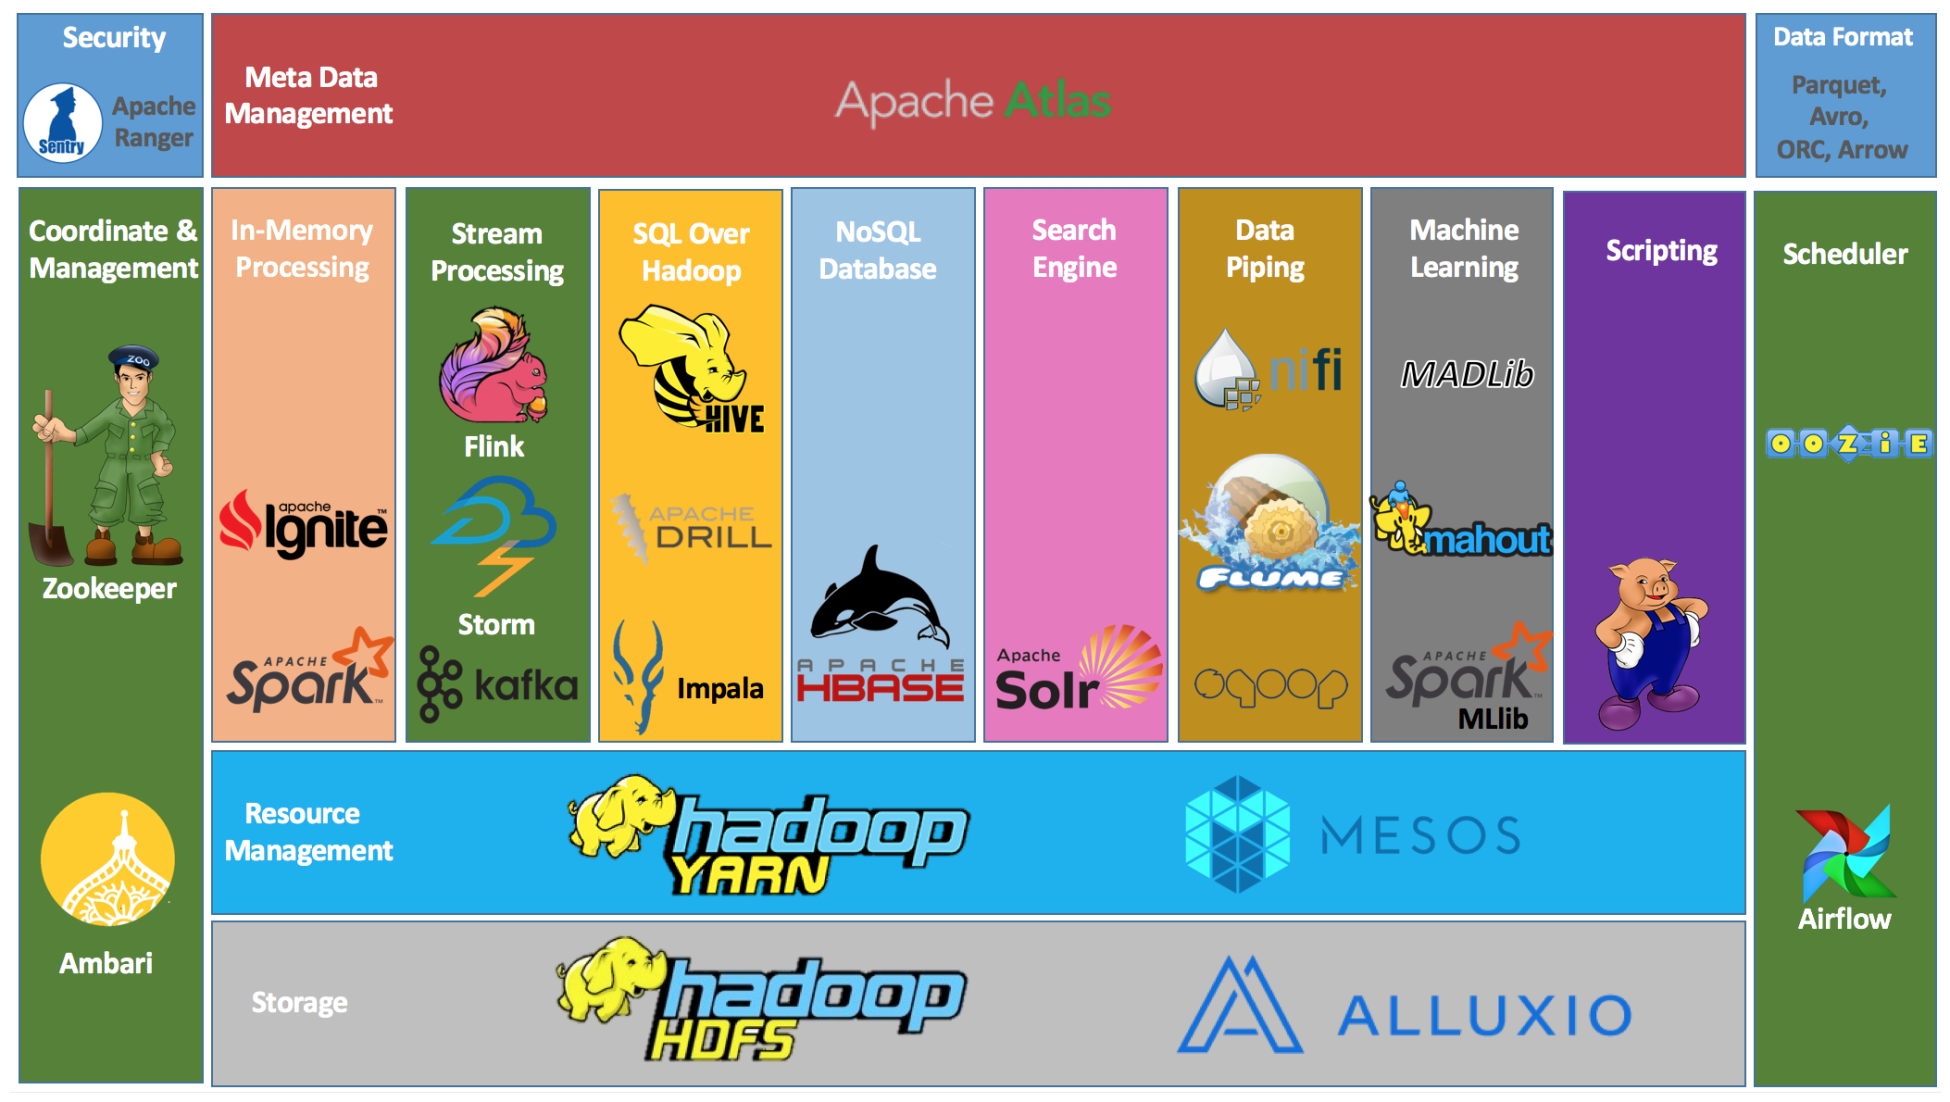
\includegraphics[width=0.7\textwidth]{hadoop_生态.png}
    \caption{hadoop生态圈\cite{hadoop_sheng}}
    \label{hadoop_shengtai}

\end{figure}
HDFS、YARN和MapReduce之间的关系非常密切。在Hadoop生态系统中,它们协同工作以提供大数据处理能力。首先,用户或应用程序将数据存储在HDFS中,然后使用MapReduce来处理这些数据。YARN负责管理和调度在集群中运行的MapReduce作业。

\subsubsection{HDFS简述}
HDFS主要是解决大数据如何存储问题的。分布式意味着是HDFS是横跨在多台计算机上的存储系统。
HDFS是一种能够在普通硬件上运行的分布式文件系统,它是高度容错的,适应于具有大数据集的应用程序,它非常适合存储大型数据(比如 TB 和 PB)。
HDFS使用多台计算机存储文件,并且提供统一的访问接口,使用户可以像访问一个普通文件系统一样使用分布式文件系统。

\begin{itemize}
\item BLOCK\\
物理磁盘中有块(Block)的概念,磁盘的物理Block是磁盘操作最小的单元。
文件系统在物理Block之上抽象了另一层概念,文件系统Block物理磁盘Block的整数倍。
HDFS的文件被拆分成block-sized的chunk,chunk作为独立单元存储。

\item Namenode与Datanode\\
图\ref{hdfs_}为HDFS的工作简图。\\
\\
NameNode主要用于维护文件系统命名空间(文件/目录树),管理元数据(Block 位置、副本数等),不存储实际数据。
而DataNode主要用于实际存储数据 Block,处理读写请求(来自客户端或 NameNode),定期向 NameNode 汇报 Block 列表。
还有Secondary NameNode 用来监控 HDFS 状态的辅助后台程序,每隔一段时间获取 HDFS 元数据的快照。最主要作用是辅助 NameNode 管理元数据信息。

\begin{figure}[htbp]
\subfloat[]{
    \label{hdfs_1}
    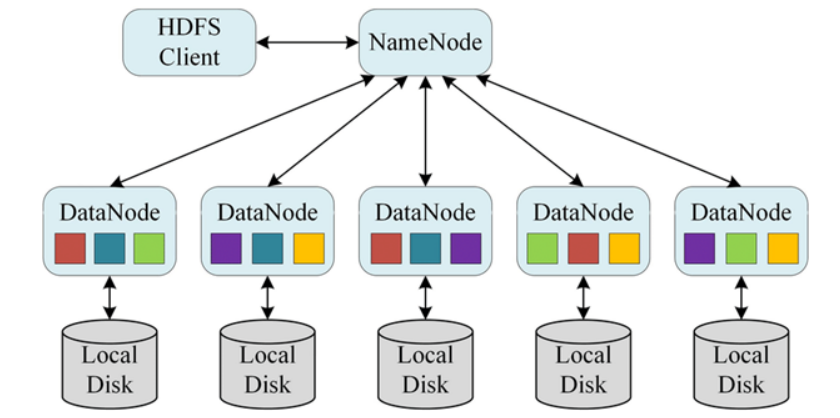
\includegraphics[width=6.77cm]{hdfs_1.png}
   
}
\subfloat[]{
    \label{hdfs_2}
    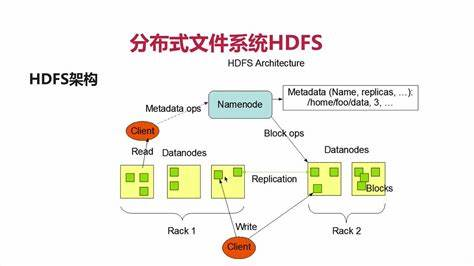
\includegraphics[width=7.04cm]{hdfs_2.png}
}
\caption{HDFS工作简图}
\label{hdfs_}
\end{figure}

\item 副本机制\\
为了容错,文件的所有block都会有副本。每个文件的block大小和副本系数都是可配置的。应用程序可以指定某个文件的副本数目。副本系数可以在文件创建的时候指定,也可以在之后改变。

\end{itemize}
\subsubsection{Yarn原理简述}
是一个通用的资源管理系统和调度平台。包括批处理、交互式查询、流处理以及其他类型的工作负载。

\begin{itemize}
    

\item 核心组件
在Hadoop集群中,YARN主要有以下几个核心组件,如图\ref{yarn_pic}:\cite{hadoop_zh}\\
- ResourceManager(资源管理器):ResourceManager是YARN集群中的主节点,负责管理整个集群的资源分配和作业调度。它跟踪可用资源,并为提交到集群的应用程序分配资源。\\
- NodeManager(节点管理器):NodeManager运行在每个集群节点上,负责管理该节点上的资源,并与ResourceManager通信以报告节点的资源使用情况和可用性。\\
- ApplicationMaster(应用程序管理器):每个提交到YARN集群的应用程序都有一个对应的ApplicationMaster。ApplicationMaster负责与ResourceManager协商资源、监控作业进度,并向ResourceManager请求更多资源或报告作业完成情况。\\
\begin{figure}[htbp]
    \centering
    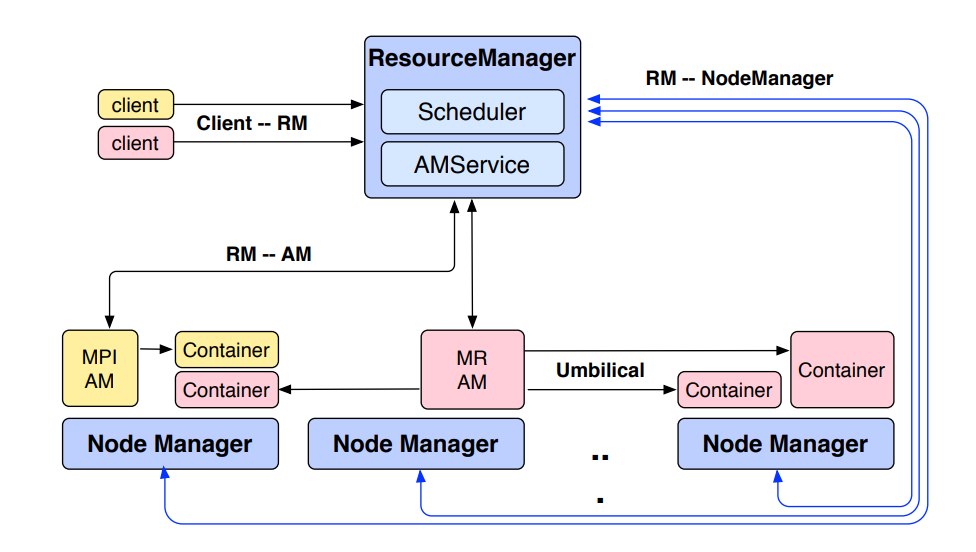
\includegraphics[width=0.7\textwidth]{yarn_pic.png}
    \caption{Yarn架构\cite{yarn}}
    \label{yarn_pic}
\end{figure}


\item 工作流程如图\ref{yarn_1}\\

\begin{figure}[htbp]
    \centering
    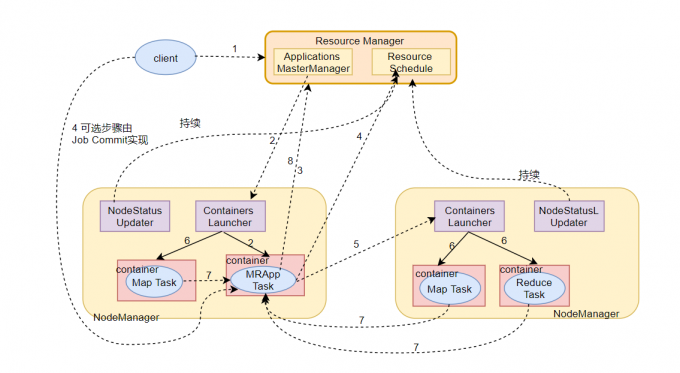
\includegraphics[width=0.8\textwidth]{yarn_1.png}
    \caption{Yarn运行流程\cite{yarns}}
    \label{yarn_1}
\end{figure}




\end{itemize}
\subsubsection{MapReduce简述}
核心思想:分而治之。将大数据集拆分为小块,分配到集群的多个节点并行处理。如图\ref{mr_all}。\\
(1) Map 阶段:将输入的大数据集切分为若干数据块,由多个Map任务并行处理。每个Map任务对数据块进行分析、过滤和转换,输出键值对作为中间结果。\\
(2) Shuffle与Sort 阶段:对Map阶段输出的所有键值对按照key进行分组和排序。该阶段会将相同key的数据聚集到一起,并将数据从Map节点传输到对应的Reduce节点,为后续归约操作做准备。\\
(3) Reduce 阶段:对Shuffle与Sort阶段分组后的数据进行归约处理。每个Reduce任务对同一key的所有value进行合并、统计或聚合,最终输出结果数据集,完成整个分布式计算过程。\\
\begin{figure}[htbp]
    \centering
    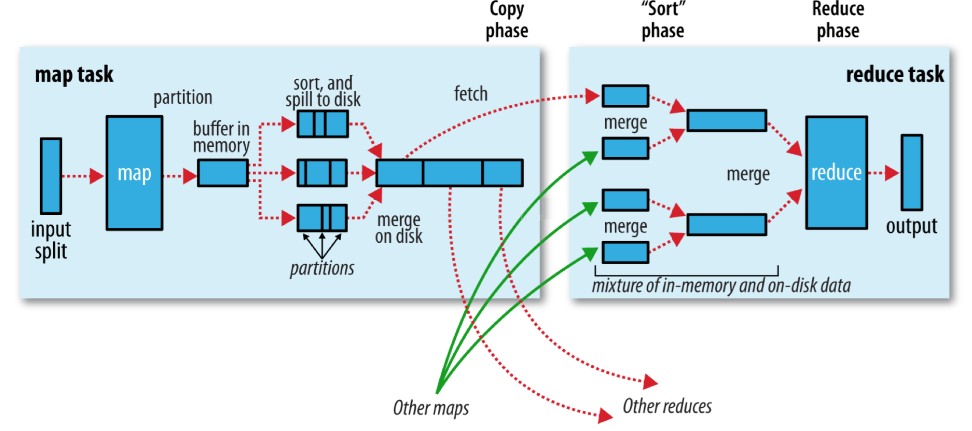
\includegraphics[width=0.7\textwidth]{mr.png}
    \vspace{1em} % 两图之间留空,可根据需要调整
    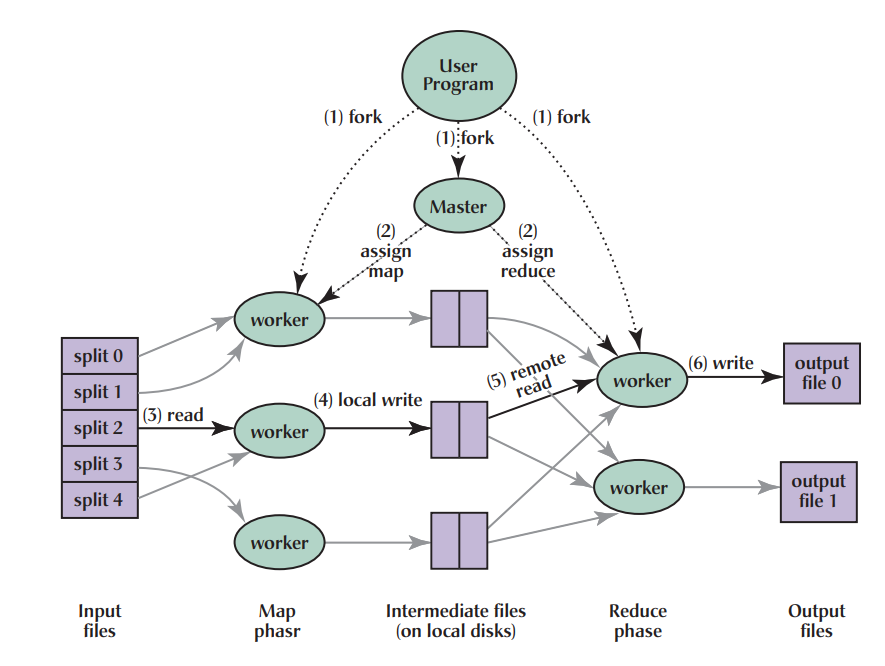
\includegraphics[width=0.7\textwidth]{mr2.png}
    \caption{MapReduce简易流程\cite{mr}\cite{mr2_heima}}
    \label{mr_all}
\end{figure}

\subsection{SpringBoot关系}
\textbf{项目结构:\cite{springboot_official}}前端向系统发起请求,首先由 controller 层 进行接收和响应处理,该层负责接口路由和基本参数校验\cite{postman_official}。随后请求被传递到 service 层,该层负责具体的业务逻辑处理。如果涉及数据库操作,service 层 会调用 mapper 层,通过 MyBatis 框架访问底层的 MySQL 数据库,完成数据的增删改查操作。
同时,service 层还可以通过 client 与 Hadoop 集群进行交互,实现分布式文件的上传、下载与删除等功能。如图\ref{sb_1}所示:

\begin{figure}[htbp]
    \centering
    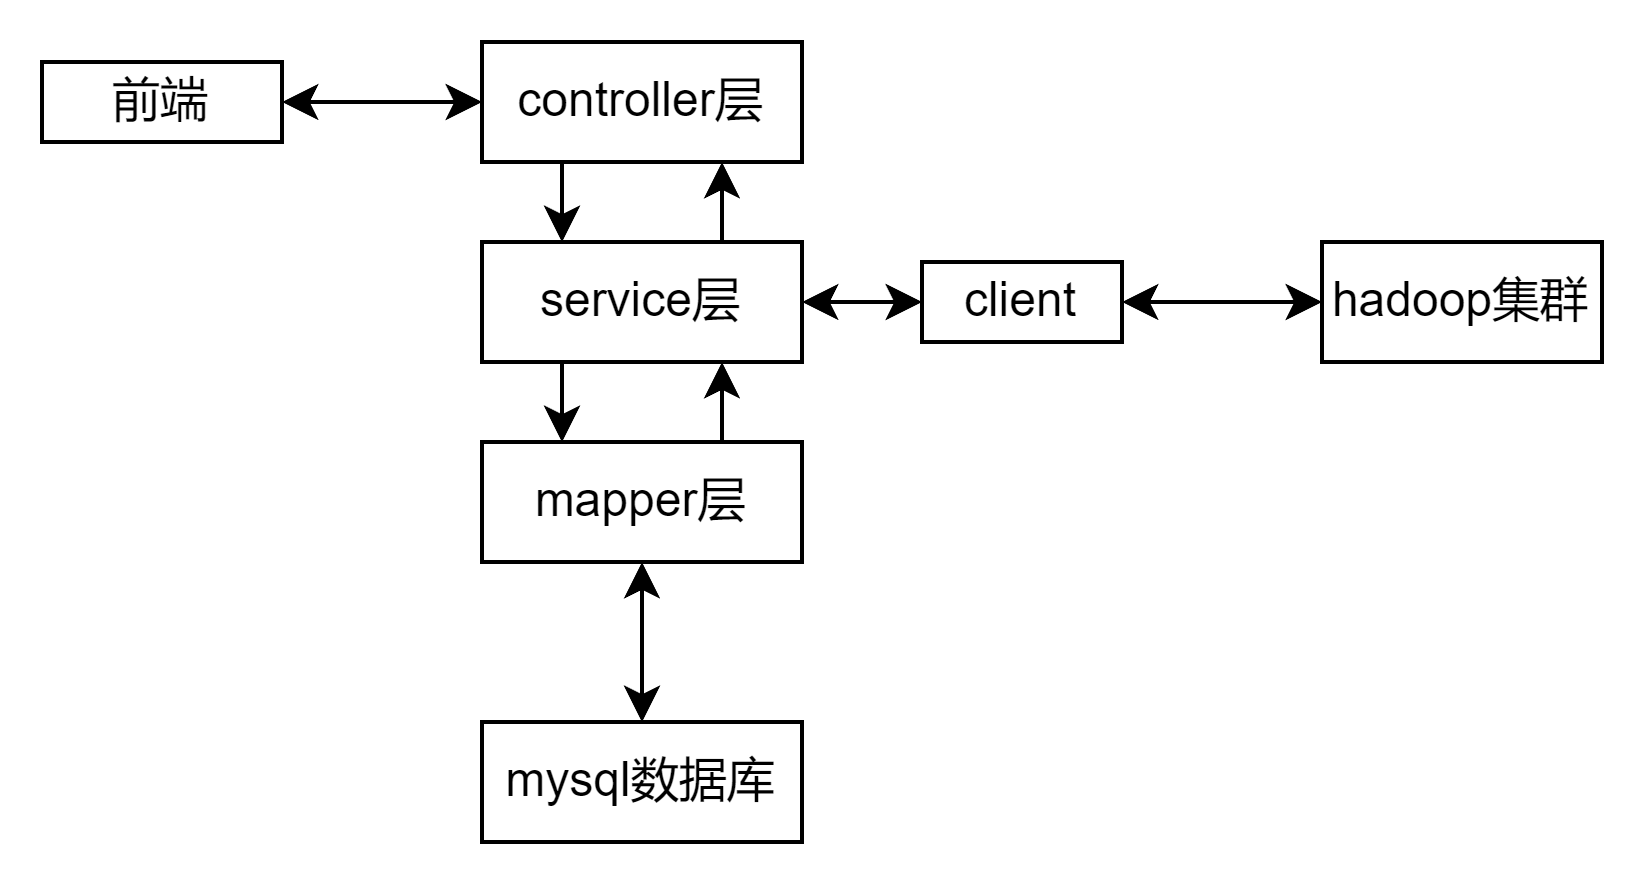
\includegraphics[width=0.7\textwidth]{sb_struct.png}
    \caption{项目结构}
    \label{sb_1}
\end{figure}



\subsection{Vue关系}
\textbf{项目结构:}

利用vue\cite{vue_official}及element\cite{element}等组件构建用户友好的可视化界面。\\
结构如图\ref{vue_struct}所示:

\begin{figure}[htbp]
    \centering
    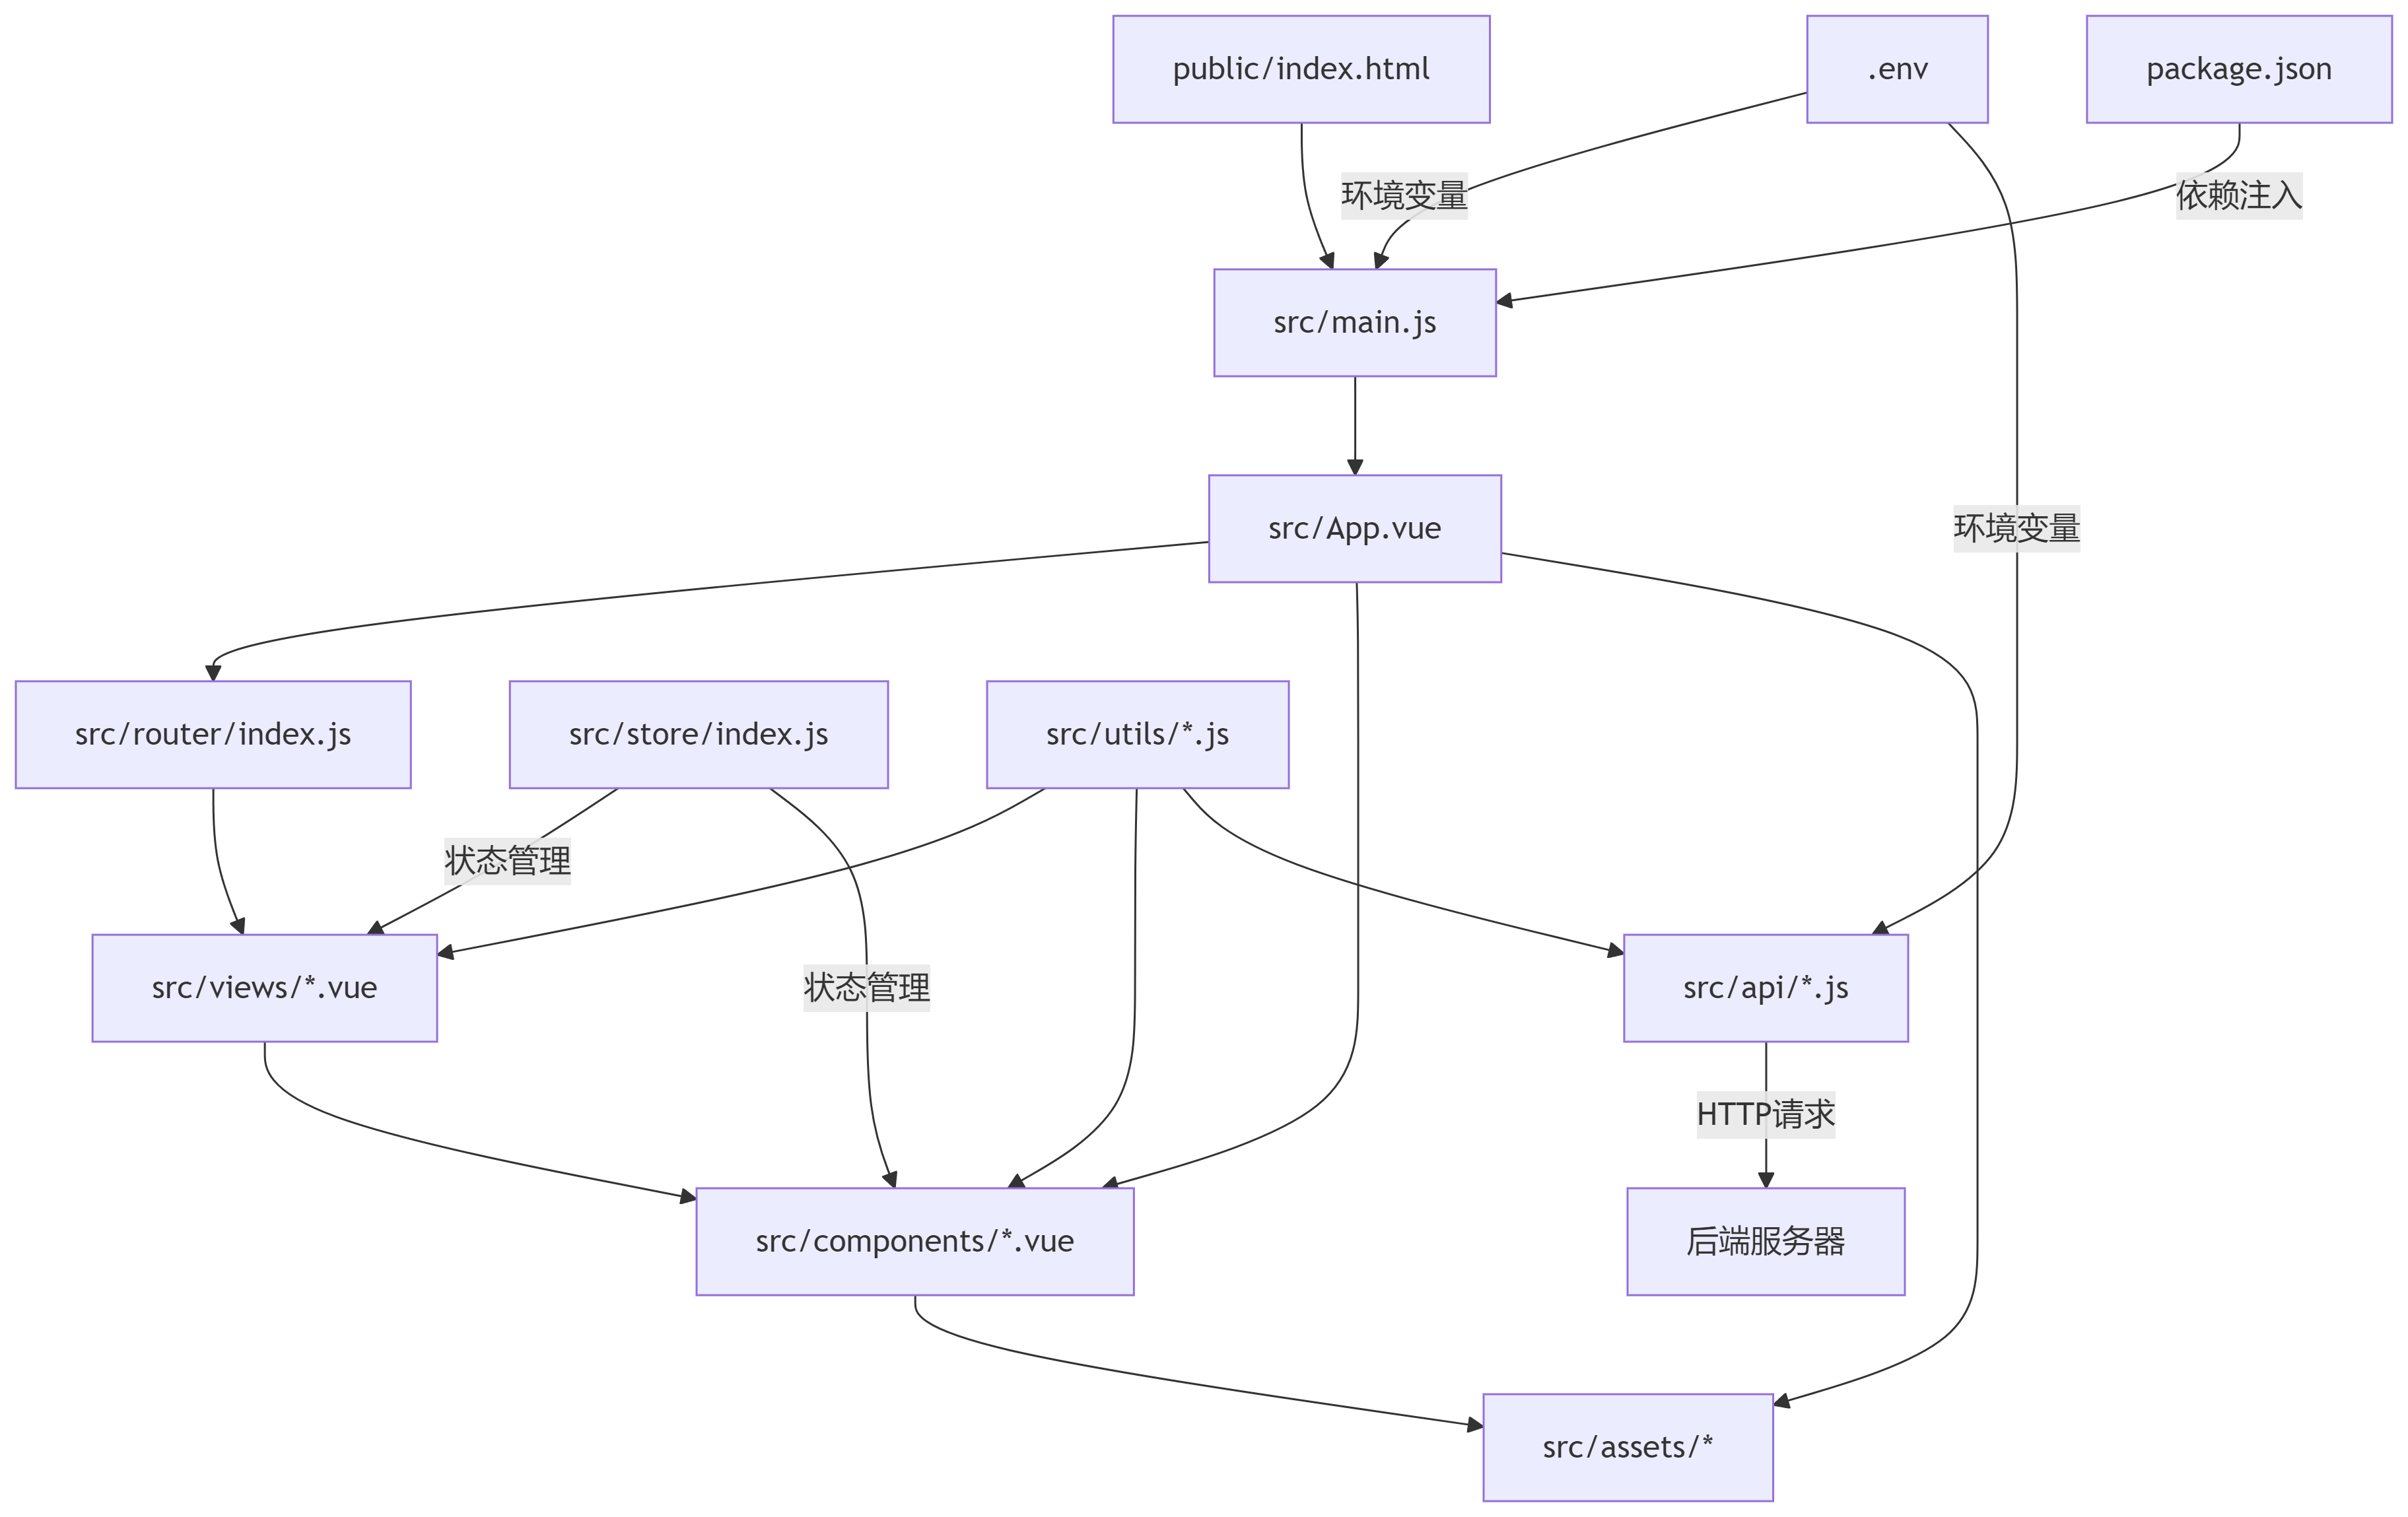
\includegraphics[width=1.0\textwidth]{vue_struct.png}
    \caption{vue结构}
    \label{vue_struct}
\end{figure}


\chapter{详细设计及实现}

\section{hadoop 集群搭建}
\subsection{配置虚拟机}
使用 VmwareWorkstation Pro,将准备好的CentOS7操作系统导入虚拟机中,配置好网络,选择NAT模式。
配置是为了确保虚拟机能够通过宿主机访问外部网络,同时宿主机也能与虚拟机通信。
详细原理见图\ref{nat}。
\begin{figure}[htbp]
    \centering
    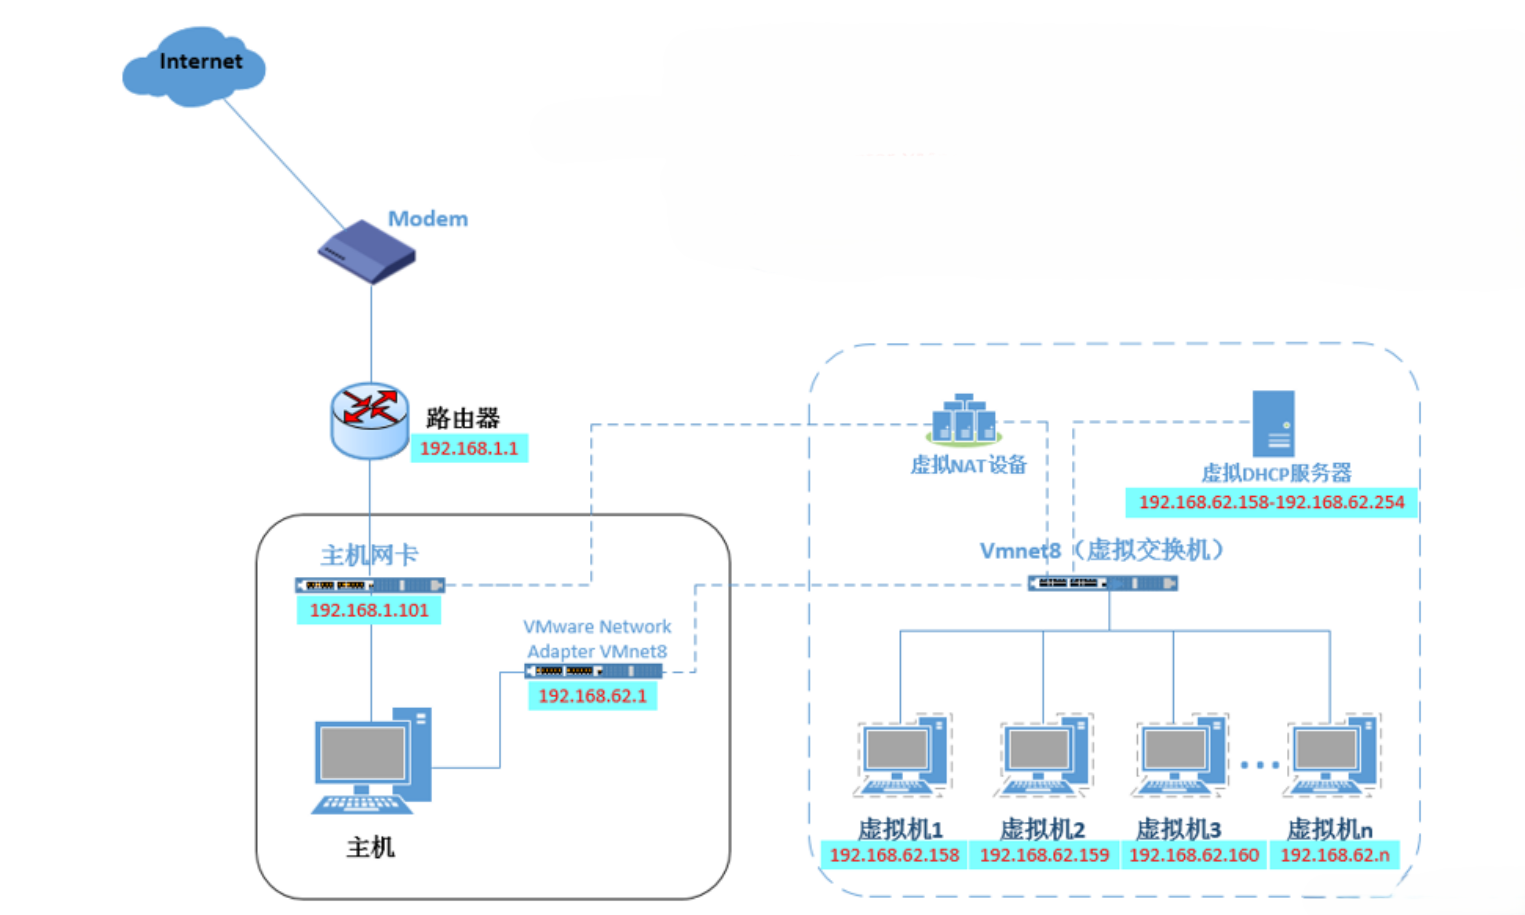
\includegraphics[width=0.7\textwidth]{nat.png}
    \caption{虚拟机网络配置}
    \label{nat}
\end{figure}
\subsection{设备配置}
\subsubsection{角色分配}
这里我们使用三个节点搭建 hadoop 集群,角色分配如表\ref{node_tables}:\\ 
\begin{table}[ht]
\centering

\begin{tabular}{|l|l|c|c|c|c|c|}
\hline
服务器 & 角色 & Namenode & Datanode & Resourcemanager & Nodemanager & SecondaryNameNode \\
\hline
node1 & Master & $\checkmark$ & $\checkmark$ & $\checkmark$ & $\checkmark$ & \\
\hline
node2 & Slaver1 &  & $\checkmark$ &  & $\checkmark$ & $\checkmark$ \\
\hline
node3 & Slaver2 &  & $\checkmark$ &  & $\checkmark$ & \\
\hline
\end{tabular}

\caption{Hadoop 集群节点角色分配}
\label{node_tables}
\end{table}

\subsubsection{Hadoop编译配置}

\begin{itemize}
\item \textbf{安装编译依赖}
\begin{verbatim}
# 1. 编译工具链
yum install -y gcc gcc-c++ make autoconf automake libtool
# 2. 压缩库支持
yum install -y lzo-devel zlib-devel snappy-devel bzip2-devel lzo 
lzo-devel lzop zlib
# 3. 其他依赖
yum install -y curl openssl openssl-devel ncurses-devel libXtst
# 4. SASL和文档
yum install -y doxygen cyrus-sasl* saslwrapper-devel*
\end{verbatim}
第一个命令:安装 编译和运行 Hadoop 的必需依赖,包括:编译工具链 、压缩库、加密和网络、其他依赖
\\第二个命令:安装 安全认证和工具。Hadoop 集群需要 Kerberos 安全认证,必须安装 SASL 相关库。
\item \textbf{安装CMake}
\begin{verbatim}
  #yum卸载已安装cmake 版本低
  yum erase cmake
  #解压
  tar zxvf CMake-3.19.4.tar.gz
  #编译安装
  cd /export/server/CMake-3.19.4
  ./configure
  make && make install
  #验证
  # cmake -version
  #如果没有正确显示版本 请断开SSH连接 重写登录
\end{verbatim}

\item \textbf{安装snappy}
\begin{verbatim}
  #卸载已经安装的
  rm -rf /usr/local/lib/libsnappy*
  rm -rf /lib64/libsnappy*
  #上传解压
  tar zxvf snappy-1.1.3.tar.gz 
  #编译安装
  cd /export/server/snappy-1.1.3
  ./configure
  make && make install
  #验证是否安装
  # ls -lh /usr/local/lib |grep snappy
\end{verbatim}


\item \textbf{配置JDK}
\begin{verbatim}
  #解压安装包
  tar zxvf jdk-8u65-linux-x64.tar.gz
  #配置环境变量
  vim /etc/profile
  export JAVA_HOME=/export/server/jdk1.8.0_241
  export PATH=$PATH:$JAVA_HOME/bin
  export CLASSPATH=.:$JAVA_HOME/lib/dt.jar:$JAVA_HOME/lib/tools.jar
  source /etc/profile
  #验证是否安装成功
  java -version
\end{verbatim}

\item \textbf{安装配置maven}
\begin{verbatim}
  #解压安装包
  tar zxvf apache-maven-3.5.4-bin.tar.gz
  #配置环境变量
  vim /etc/profile
  export MAVEN_HOME=/export/server/apache-maven-3.5.4
  export MAVEN_OPTS="-Xms4096m -Xmx4096m"
  export PATH=:$MAVEN_HOME/bin:$PATH
  source /etc/profile
  #验证是否安装成功
  # mvn -v
  #添加maven 阿里云仓库地址 加快编译速度
  vim /export/server/apache-maven-3.5.4/conf/settings.xml
    <mirrors>
    <mirror>
    <id>alimaven</id>
    <name>aliyun maven</name>
    <url>http://maven.aliyun.com/nexus/content/groups/public/</url>
    <mirrorOf>central</mirrorOf>
    </mirror>
    </mirrors>
\end{verbatim}

\item \textbf{安装ProtocolBuffer}
\begin{verbatim}
  #解压
  tar zxvf protobuf-3.7.1.tar.gz
  #编译安装
  cd /export/server/protobuf-3.7.1
  ./autogen.sh
  ./configure
  make && make install
  #验证是否安装成功
  # protoc --version
\end{verbatim}

\item \textbf{编译hadoop}
\begin{verbatim}
  #上传解压源码包
  tar zxvf hadoop-3.3.0-src.tar.gz
  #编译
  cd /root/hadoop-3.3.0-src
  mvn clean package -Pdist,native -DskipTests -Dtar -Dbundle.snappy
    -Dsnappy.lib=/usr/local/lib
  #参数说明:
  Pdist,native :把重新编译生成的hadoop动态库;
  DskipTests :跳过测试
  Dtar :最后把文件以tar打包
  Dbundle.snappy :添加snappy压缩支持【默认官网下载的是不支持的】
  Dsnappy.lib=/usr/local/lib :指snappy在编译机器上安装后的库路径
\end{verbatim}

\item \textbf{编译之后的安装包路径}
\begin{verbatim}
/root/hadoop-3.3.0-src/hadoop-dist/target
\end{verbatim}
\end{itemize}

\subsubsection{Hadoop集群分布式安装}
将集群的环境全部编译完成之后,对一台机器进行配置,然后利用scp命令可以分发到其他机器上。
\begin{itemize}
\item \textbf{配置主机映射}
\begin{verbatim}
vi /etc/hosts 命令修改主机映射
\end{verbatim}


\item \textbf{JDK安装与环境变量}
\begin{verbatim}
#配置环境变量
vim /etc/profile
export JAVA_HOME=/export/server/jdk1.8.0_241
export PATH=$PATH:$JAVA_HOME/bin
export CLASSPATH=.:$JAVA_HOME/lib/dt.jar:$JAVA_HOME/lib/tools.jar
#重新加载环境变量文件
source /etc/profile
\end{verbatim}

\item \textbf{系统配置}
\begin{verbatim}
# 集群时间同步
ntpdate ntp5.aliyun.com
# 防火墙关闭
firewall-cmd --state	#查看防火墙状态
systemctl stop firewalld.service  #停止firewalld服务
systemctl disable firewalld.service  #开机禁用firewalld服务
# systemctl status firewalld.service
#创建统一目录
mkdir -p /export/server #软件安装路径
mkdir -p /export/data #数据存储路径
mkdir -p /export/software/ #安装包存储路径
\end{verbatim}

\item \textbf{SSH免密登录}
\begin{verbatim}
# ssh免密登录(只需要配置node1至node1、node2、node3即可)
  	#node1生成公钥私钥
  	ssh-keygen  
  	#node1配置免密登录到node1 node2 node3
  	ssh-copy-id node1
  	ssh-copy-id node2
  	ssh-copy-id node3
\end{verbatim}

\item \textbf{上传Hadoop安装包}
\begin{verbatim}
  hadoop-3.3.0-Centos7-64-with-snappy.tar.gz
  tar zxvf hadoop-3.3.0-Centos7-64-with-snappy.tar.gz
\end{verbatim}

\item \textbf{修改配置文件}
\\
hadoop-env.sh:
\begin{verbatim}
    #文件最后添加
    export JAVA_HOME=/export/server/jdk1.8.0_241
    export HDFS_NAMENODE_USER=root
    export HDFS_DATANODE_USER=root
    export HDFS_SECONDARYNAMENODE_USER=root
    export YARN_RESOURCEMANAGER_USER=root
    export YARN_NODEMANAGER_USER=root 
\end{verbatim}
core-site.xml:
\begin{verbatim}
    <property>
        <name>fs.defaultFS</name>
        <value>hdfs://node1:8020</value>
    </property>
    <!-- 设置Hadoop本地保存数据路径 -->
    <property>
        <name>hadoop.tmp.dir</name>
        <value>/export/data/hadoop-3.3.0</value>
    </property>
    <!-- 设置HDFS web UI用户身份 -->
    <property>
        <name>hadoop.http.staticuser.user</name>
        <value>root</value>
    </property>
    <!-- 整合hive 用户代理设置 -->
    <property>
        <name>hadoop.proxyuser.root.hosts</name>
        <value>*</value>
    </property>
    <property>
        <name>hadoop.proxyuser.root.groups</name>
        <value>*</value>
    </property>
    <!-- 文件系统垃圾桶保存时间 -->
    <property>
        <name>fs.trash.interval</name>
        <value>1440</value>
    </property>
\end{verbatim}
hdfs-site.xml:
\begin{verbatim}
    <!-- 设置SNN进程运行机器位置信息 -->
    <property>
        <name>dfs.namenode.secondary.http-address</name>
        <value>node2:9868</value>
    </property>
\end{verbatim}
mapred-site.xml:
\begin{verbatim}
    <!-- 设置MR程序默认运行模式: yarn集群模式 local本地模式 -->
    <property>
      <name>mapreduce.framework.name</name>
      <value>yarn</value>
    </property>
    <!-- MR程序历史服务地址 -->
    <property>
      <name>mapreduce.jobhistory.address</name>
      <value>node1:10020</value>
    </property>
    <!-- MR程序历史服务器web端地址 -->
    <property>
      <name>mapreduce.jobhistory.webapp.address</name>
      <value>node1:19888</value>
    </property>
    <property>
      <name>yarn.app.mapreduce.am.env</name>
      <value>HADOOP_MAPRED_HOME=${HADOOP_HOME}</value>
    </property>
    <property>
      <name>mapreduce.map.env</name>
      <value>HADOOP_MAPRED_HOME=${HADOOP_HOME}</value>
    </property>
    <property>
      <name>mapreduce.reduce.env</name>
      <value>HADOOP_MAPRED_HOME=${HADOOP_HOME}</value>
    </property>
\end{verbatim}
yarn-site.xml:
\begin{verbatim}
        <!-- 设置YARN集群主角色运行机器位置 -->
    <property>
    	<name>yarn.resourcemanager.hostname</name>
    	<value>node1</value>
    </property>
    <property>
        <name>yarn.nodemanager.aux-services</name>
        <value>mapreduce_shuffle</value>
    </property>
    <!-- 是否将对容器实施物理内存限制 -->
    <property>
        <name>yarn.nodemanager.pmem-check-enabled</name>
        <value>false</value>
    </property>
    <!-- 是否将对容器实施虚拟内存限制。 -->
    <property>
        <name>yarn.nodemanager.vmem-check-enabled</name>
        <value>false</value>
    </property>
    <!-- 开启日志聚集 -->
    <property>
      <name>yarn.log-aggregation-enable</name>
      <value>true</value>
    </property>
    <!-- 设置yarn历史服务器地址 -->
    <property>
        <name>yarn.log.server.url</name>
        <value>http://node1:19888/jobhistory/logs</value>
    </property>
    <!-- 历史日志保存的时间 7天 -->
    <property>
      <name>yarn.log-aggregation.retain-seconds</name>
      <value>604800</value>
    </property>
\end{verbatim}
编辑hadoop配置文件workers:
\begin{verbatim}
    #配置从节点
    node1
    node2
    node3
\end{verbatim}



\item \textbf{分发同步安装包}
\begin{verbatim}
  cd /export/server
  scp -r hadoop-3.3.0 root@node2:$PWD
  scp -r hadoop-3.3.0 root@node3:$PWD
\end{verbatim}
\item \textbf{hadoop添加到环境变量(所有机器)}
\begin{verbatim}
  vim /etc/profile

  export HADOOP_HOME=/export/server/hadoop-3.3.0
  export PATH=$PATH:$HADOOP_HOME/bin:$HADOOP_HOME/sbin

  source /etc/profile
  #scp给其他机器!
  scp /etc/profile root@node2:/etc/
  scp /etc/profile root@node3:/etc/

  #重新加载验证
  source /etc/profile
  hadoop #验证环境变量是否生效
\end{verbatim}

图\ref{hadoop_check}为三台机器的hadoop环境的验证
\begin{figure}[htbp]
    \centering
    \subfloat[node1]{
        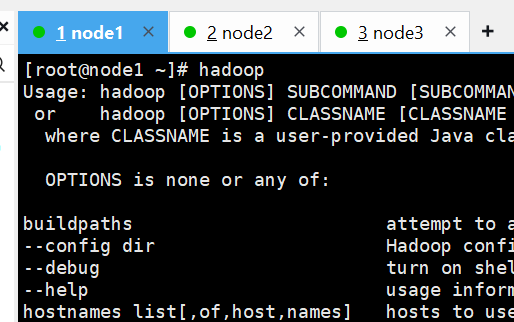
\includegraphics[height=3.5cm]{hadoop1.png}
        \label{fig:hadoop1}
    }
    \subfloat[node2]{
        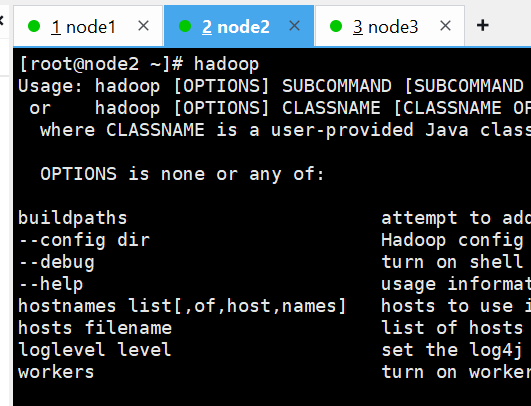
\includegraphics[height=3.5cm]{hadoop2.png}
        \label{fig:hadoop2}
    }
    \subfloat[node3]{
        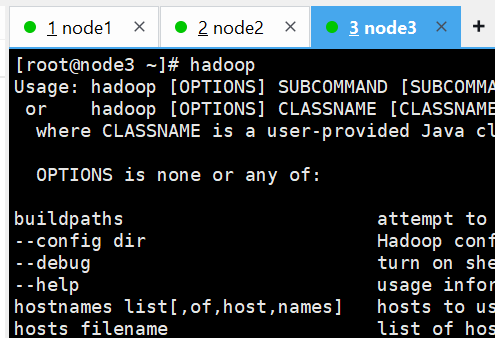
\includegraphics[height=3.5cm]{hadoop3.png}
        \label{fig:hadoop3}
    }
    \caption{Hadoop集群各节点示意图}
    \label{hadoop_check}
\end{figure}

\item \textbf{hadoop初始化(注意只执行一次!)}
首次启动HDFS时,必须对其进行格式化操作。format本质上是初始化工作,进行HDFS清理和准备工作
\begin{verbatim}
hdfs namenode -format
\end{verbatim}
\end{itemize}


\subsection{Hadoop集群启动与使用}

\subsubsection{启动Hadoop集群}
\begin{verbatim}
#HDFS集群
start-dfs.sh
stop-dfs.sh
#YARN集群
start-yarn.sh
stop-yarn.sh
#Hadoop集群
start-all.sh
stop-all.sh 
\end{verbatim}
一般利用:start-all.sh可以直接全部启动

可以看到yarn如图\ref{yarn_check}和hdfs如图\ref{hdfs_file}都已经启动成功了。
\begin{figure}[htbp]
\subfloat[node1:8088]{
    \label{yarn_check}
    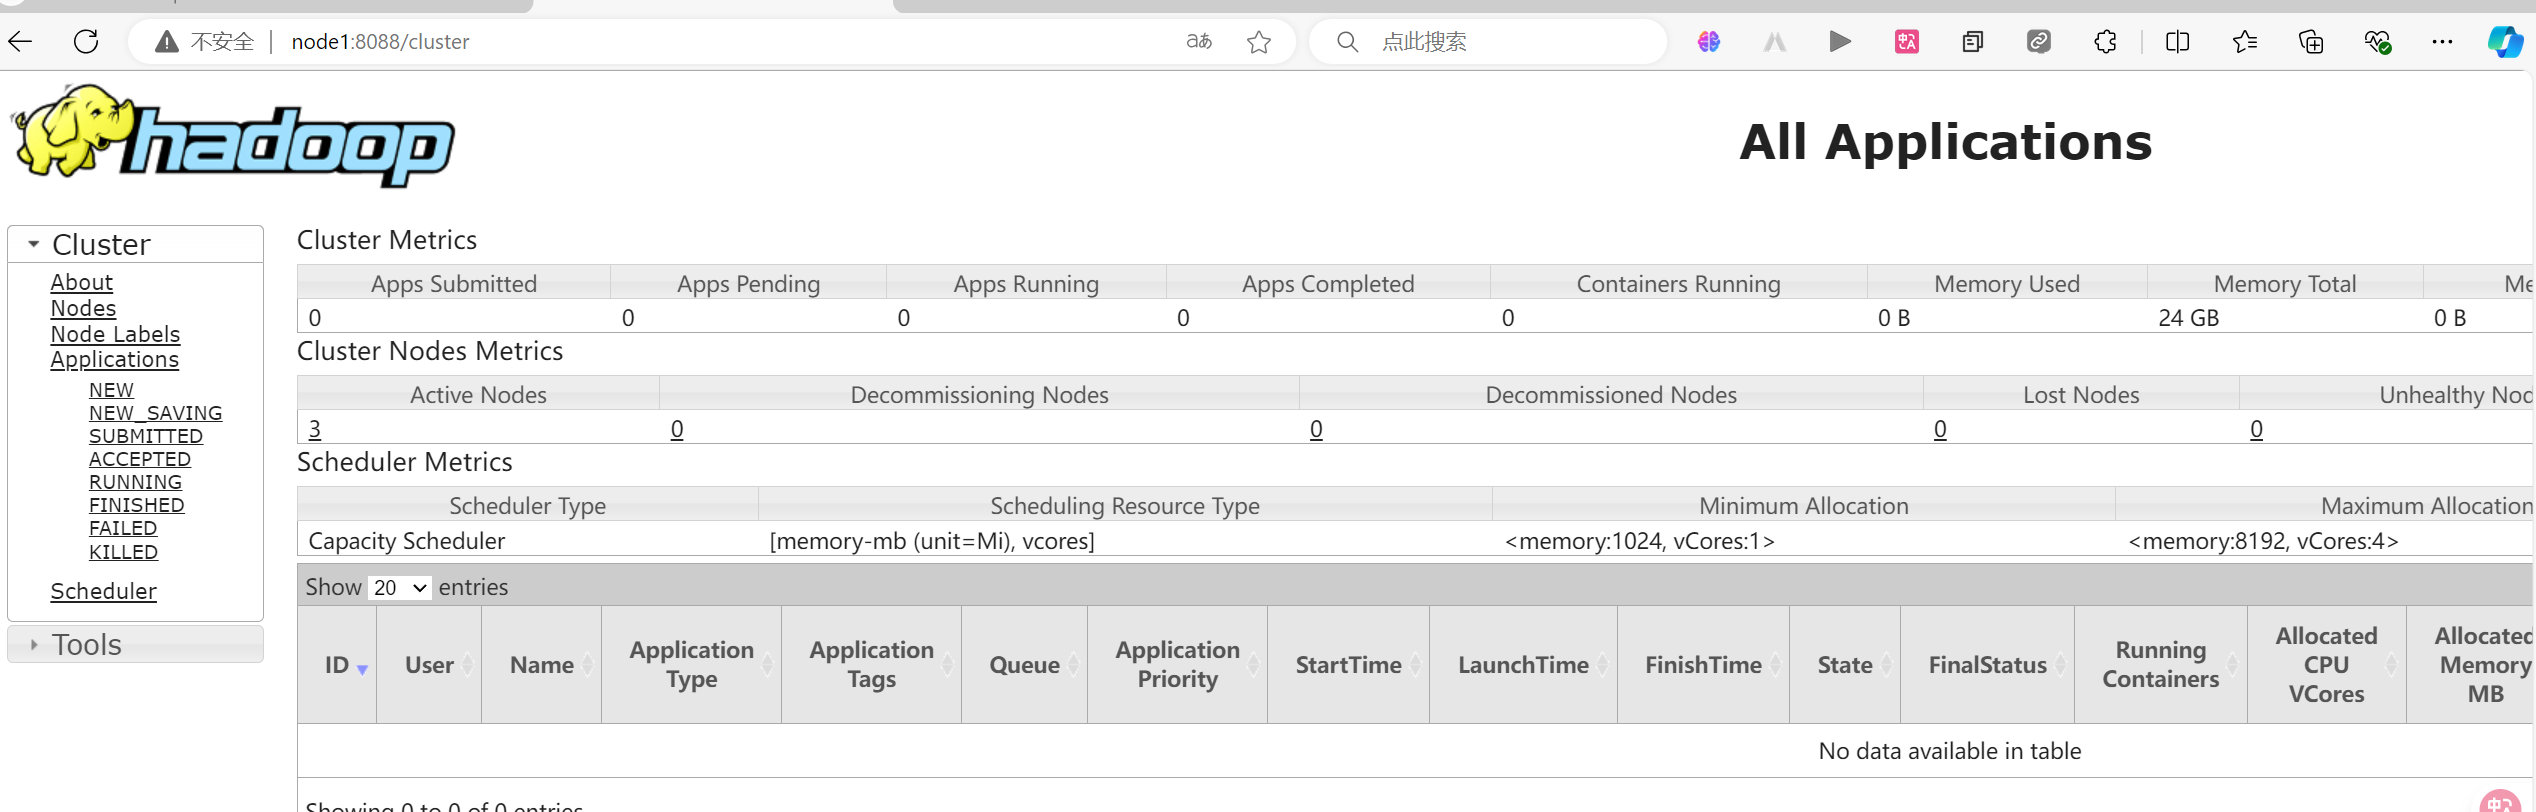
\includegraphics[width=6.77cm]{yarn_check.png}
}
\subfloat[node1:9870]{
    \label{hdfs_file}
    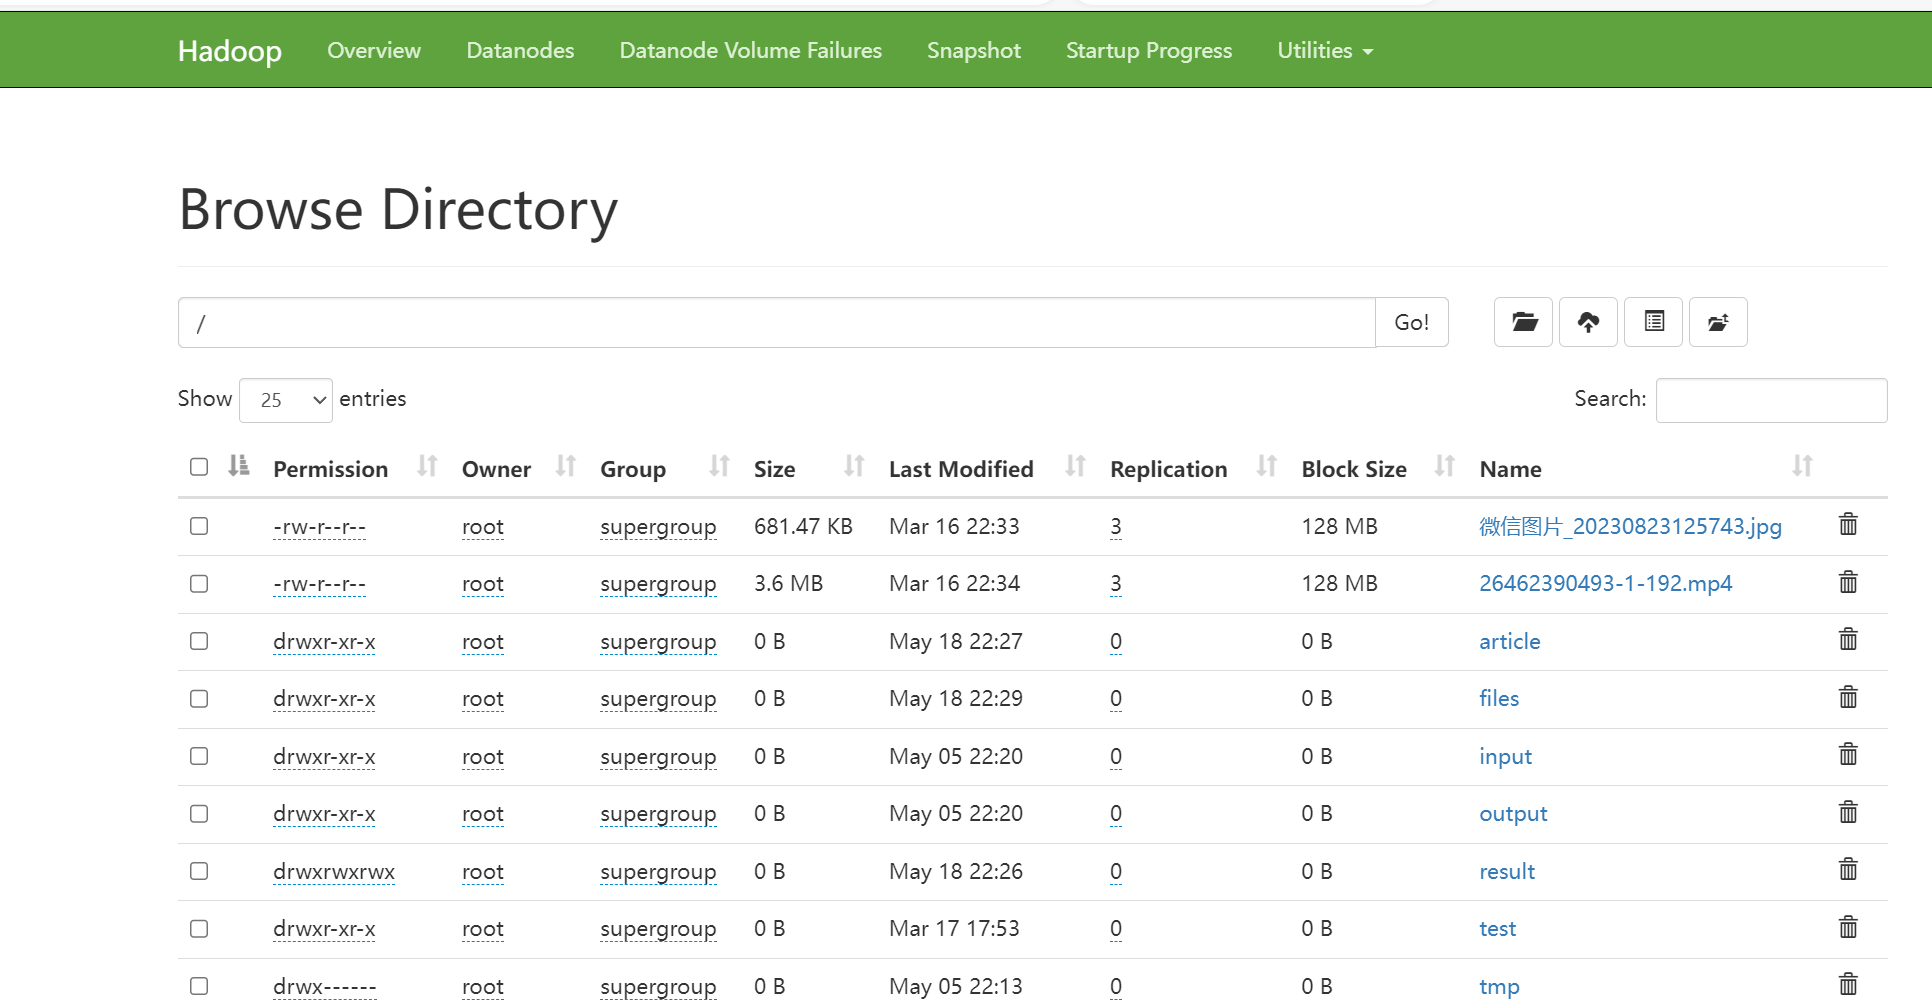
\includegraphics[width=7.04cm]{hdfs_file.png}   
}
\caption{可视化界面}
\label{check}
\end{figure}

\subsubsection{Hadoop常用指令}
\begin{itemize}
\item 创建文件夹
\begin{verbatim}
hadoop fs -mkdir [-p] <path> 
# path 为待创建的目录
# -p选项的行为与Unix mkdir -p非常相似,它会沿着路径创建父目录。
\end{verbatim}
\item 查看指定目录下内容
\begin{verbatim}
hadoop fs -ls [-h] [-R] [<path> ...]
# path 指定目录路径
# -h 人性化显示文件size
# -R 递归查看指定目录及其子目录
\end{verbatim}

\item 上传文件
\begin{verbatim}
hadoop fs -put [-f] [-p] <localsrc> ... <dst>
# -f 覆盖目标文件(已存在下)
# -p 保留访问和修改时间,所有权和权限。
# localsrc 本地文件系统(客户端所在机器)
# dst 目标文件系统(HDFS)
\end{verbatim}

\item 查看HDFS文件内容
\begin{verbatim}
hadoop fs -cat <src> ...
# 读取指定文件全部内容,显示在标准输出控制台。
# 注意:对于大文件内容读取,慎重。
\end{verbatim}

\item 下载HDFS文件
\begin{verbatim}
hadoop fs -get [-f] [-p] <src> ... <localdst>
# 下载文件到本地文件系统指定目录, localdst必须是目录
# -f 覆盖目标文件(已存在下)
# -p 保留访问和修改时间,所有权和权限。
\end{verbatim}
\item HDFS数据移动
\begin{verbatim}
hadoop fs -mv <src> ... <dst>
# 移动文件到指定文件夹下
# 可以使用该命令移动数据,重命名文件的名称
\end{verbatim}

\end{itemize}



\section{后端服务器搭建}
基于 Spring Boot 框架的后端系统架构,采用了标准的分层设计模式,包括 Controller 层、Service 层、Service 实现层(Impl)、Mapper 层,并集成了本地缓存和 Hadoop 分布式存储系统,形成了清晰、高内聚低耦合的系统结构。
后端结构如图\ref{sb_2}所示,文件结构如图\ref{sb_s}所示。
\begin{figure}[htbp]
    \centering
    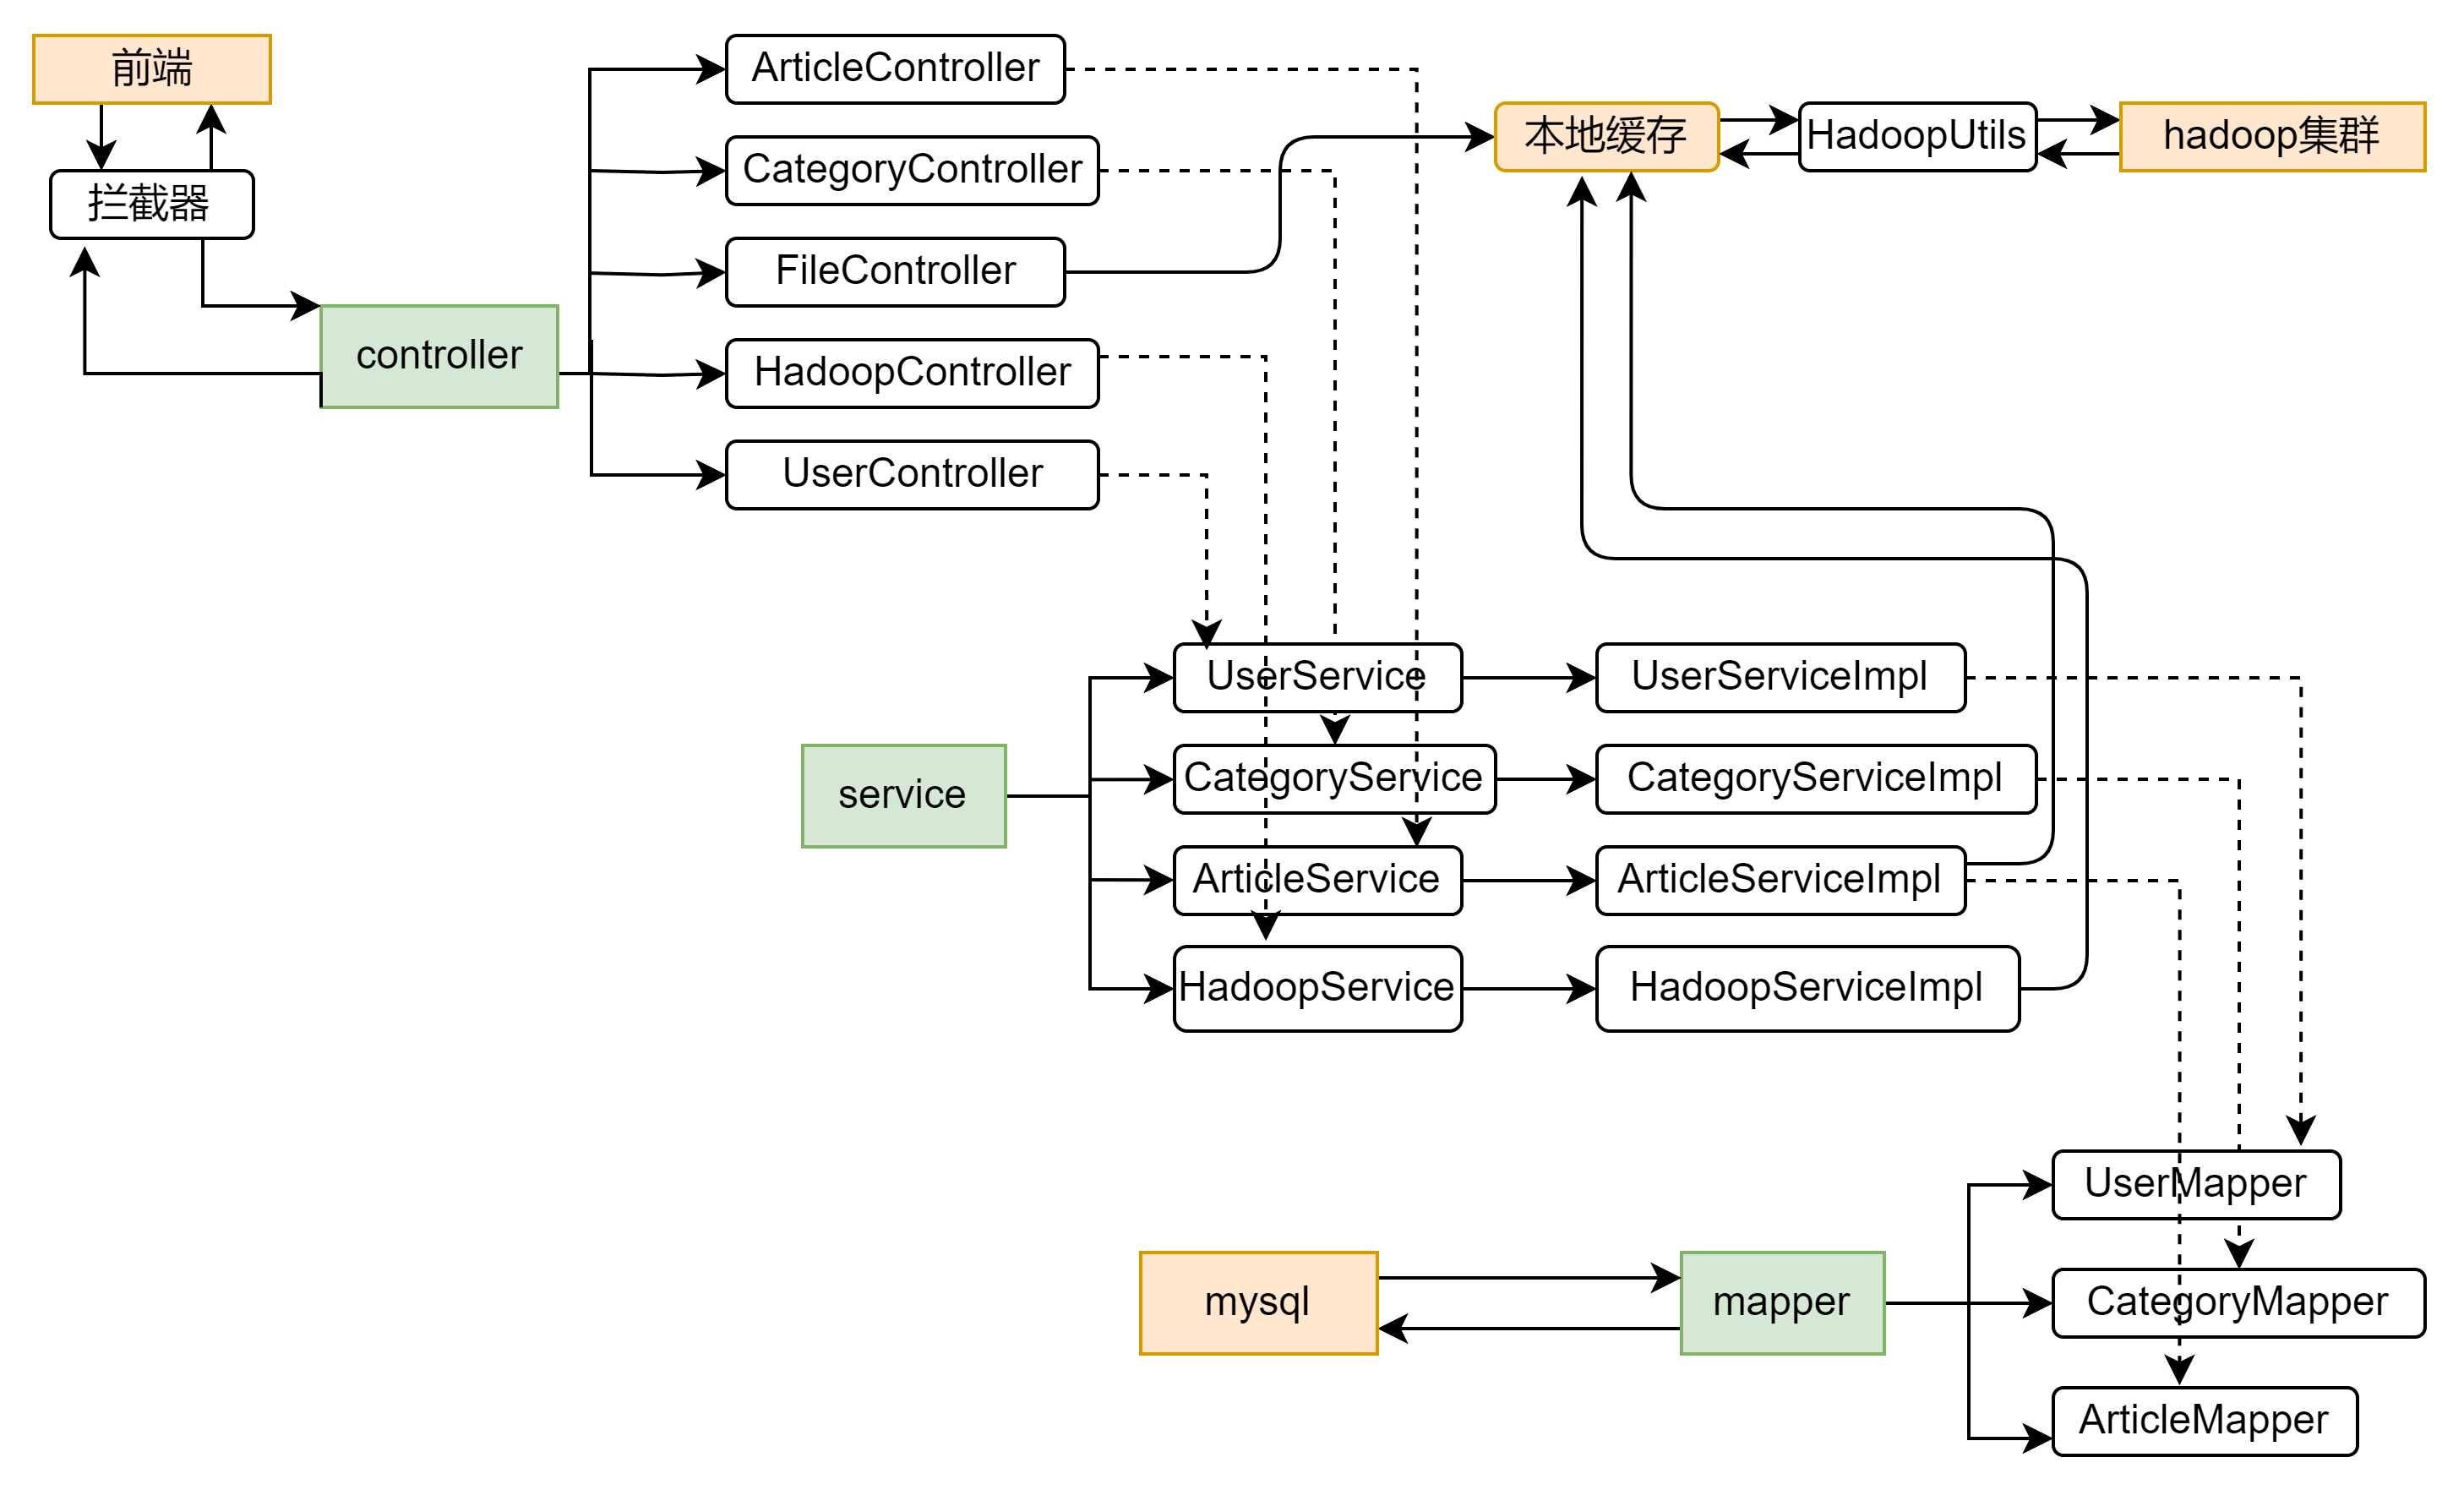
\includegraphics[width=1.0\textwidth]{sb_detail.png}
    \caption{后端结构细节}
    \label{sb_2}
\end{figure}
项目文件结构如图\ref{sb_s}所示,主要涉及登录拦截器、HTTP请求处理、数据库交互、业务逻辑、工具类、WordCount作业(可能是数据处理任务)、启动类、配置文件以及环境依赖项。
\begin{figure}[htbp]
    \centering
    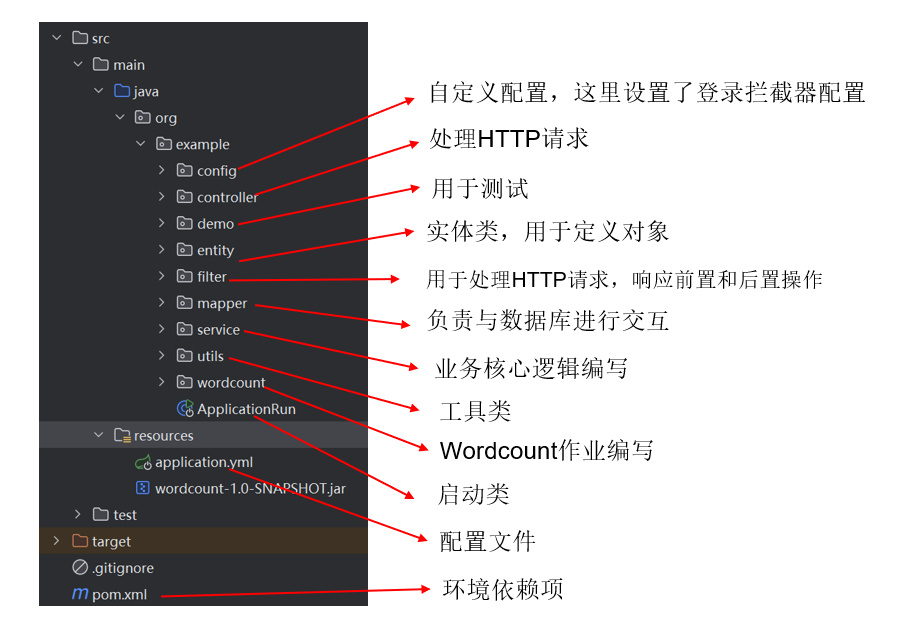
\includegraphics[width=0.7\textwidth]{sb_file_struct.png}
    \caption{后端文件结构}
    \label{sb_s}
\end{figure}
\subsection{环境搭建}
\begin{itemize}
    \item 配置 application.yaml
    如图\ref{yml}所示
    \begin{figure}[htbp]
    \centering
    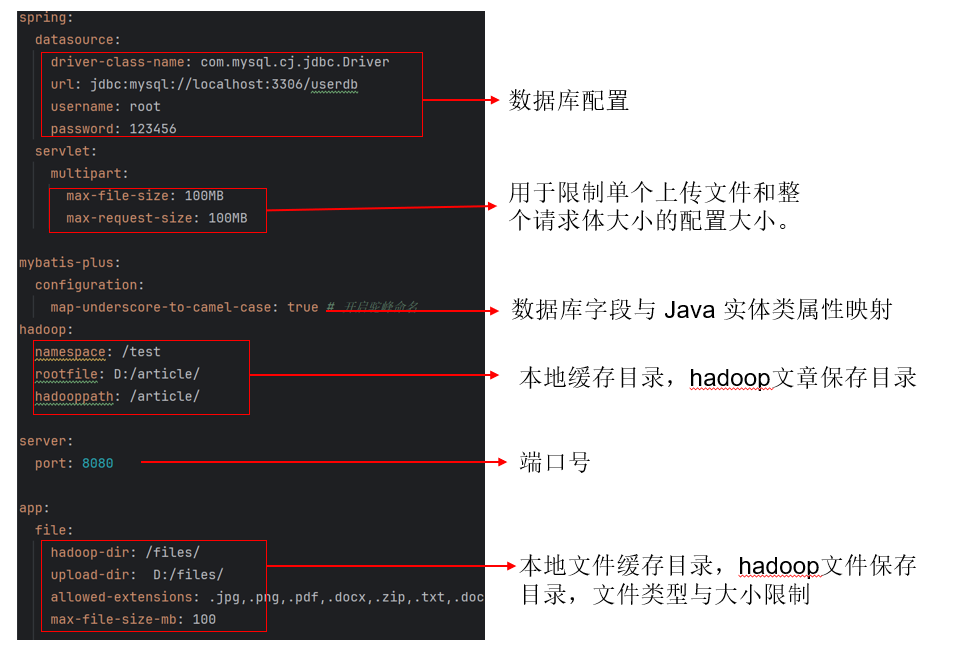
\includegraphics[width=0.7\textwidth]{yml.png}
    \caption{yml配置}
    \label{yml}
\end{figure}
    \item pom.xml
    引入依赖项:
    \begin{itemize}
    \item spring-boot-starter-web:Spring Boot Web开发的基础依赖,包含Spring MVC和嵌入式Tomcat。
    \item mybatis-plus-spring-boot3-starter:MyBatis-Plus的Spring Boot集成,简化MyBatis开发。
    \item mysql-connector-j:MySQL数据库驱动。
    \item lombok:简化Java代码,自动生成getter/setter等。
    \item spring-boot-starter-validation:参数校验支持。
    \item java-jwt:JWT生成与解析。
    \item spring-boot-starter-test:Spring Boot测试依赖。
    \item pagehelper-spring-boot-starter:MyBatis分页插件。
    \item jaxb-api、activation、jaxb-runtime:Java XML绑定相关依赖。
    \item spring-boot-starter-data-redis:Spring Boot集成Redis。
    \item jackson-databind:JSON序列化与反序列化。
    \item jsoup:HTML解析工具。
    \item javax.annotation-api:Java注解支持。
    \item commons-lang3:Apache常用工具类库。
    \item jsch:SSH协议支持。
    \item hadoop-common、hadoop-hdfs:Hadoop核心依赖和HDFS支持。
    \end{itemize}
 \item 构建数据库表\\
 如图\ref{db}所示,构建三个数据库表,分别为用户表、文章表和文件表。例如,图\ref{userdb}为用户表的具体内容。


\begin{figure}[htbp]
    \centering % 居中对齐
    \subfloat[数据库表\label{db}]{ % 子图1
        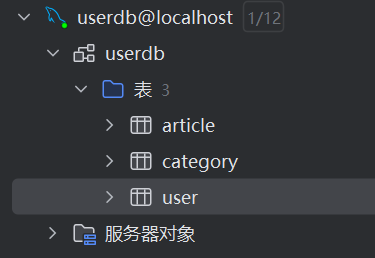
\includegraphics[width=4.55cm,height=3.5cm]{db.png}
    }
    \hfill % 添加水平填充
    \subfloat[用户表\label{userdb}]{ % 子图2
        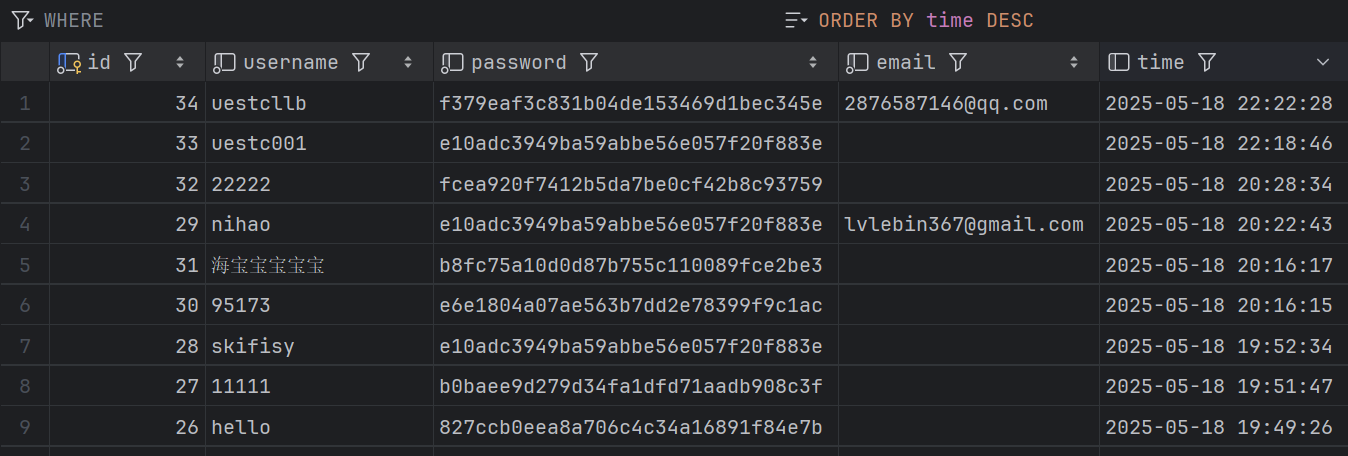
\includegraphics[width=9.04cm,height=3.5cm]{userdb.png}   
    }
    \caption{数据库表} % 总标题
    \label{dbdb} % 总标签
\end{figure}

\item 与hadoop建立client连接
在HadoopUtils里面编写函数
\begin{lstlisting}[language=Java]
// 获取 HDFS 客户端
public FileSystem getFileSystem() throws Exception {
    System.setProperty("HADOOP_USER_NAME", "root");
    Configuration conf = new Configuration();
    conf.set("fs.defaultFS", "hdfs://mycluster/");
    conf.set("dfs.nameservices", "mycluster");
    conf.set("dfs.ha.namenodes.mycluster", "nn1,nn2");
    conf.set("dfs.namenode.rpc-address.mycluster.nn1", "192.168.88.151:8020");
    conf.set("dfs.namenode.rpc-address.mycluster.nn2", "192.168.88.152:8020");
    conf.set("dfs.client.failover.proxy.provider.mycluster", "org.apache.hadoop.hdfs.server.namenode.ha.ConfiguredFailoverProxyProvider");
    return FileSystem.get(conf);
}

\end{lstlisting}
\end{itemize}

\subsection{用户登录注册}
\subsubsection{注册}

我们想要实现注册逻辑,首先在 controller 层,写一下主要的控制单元
(register),里面是主体逻辑:判断用户是否存在,存在返回 result.error,
不存在那么添加数据。
添加数据的逻辑就会调用 sevice 层,service 层主要是用来实现服务,有
两个服务,查询是否名字重复和将数据添加到数据库,那么我们再服务
层就需要 mapper 层的对于数据库的操作。
如图\ref{re}所示。
\begin{figure}[htbp]
    \centering
    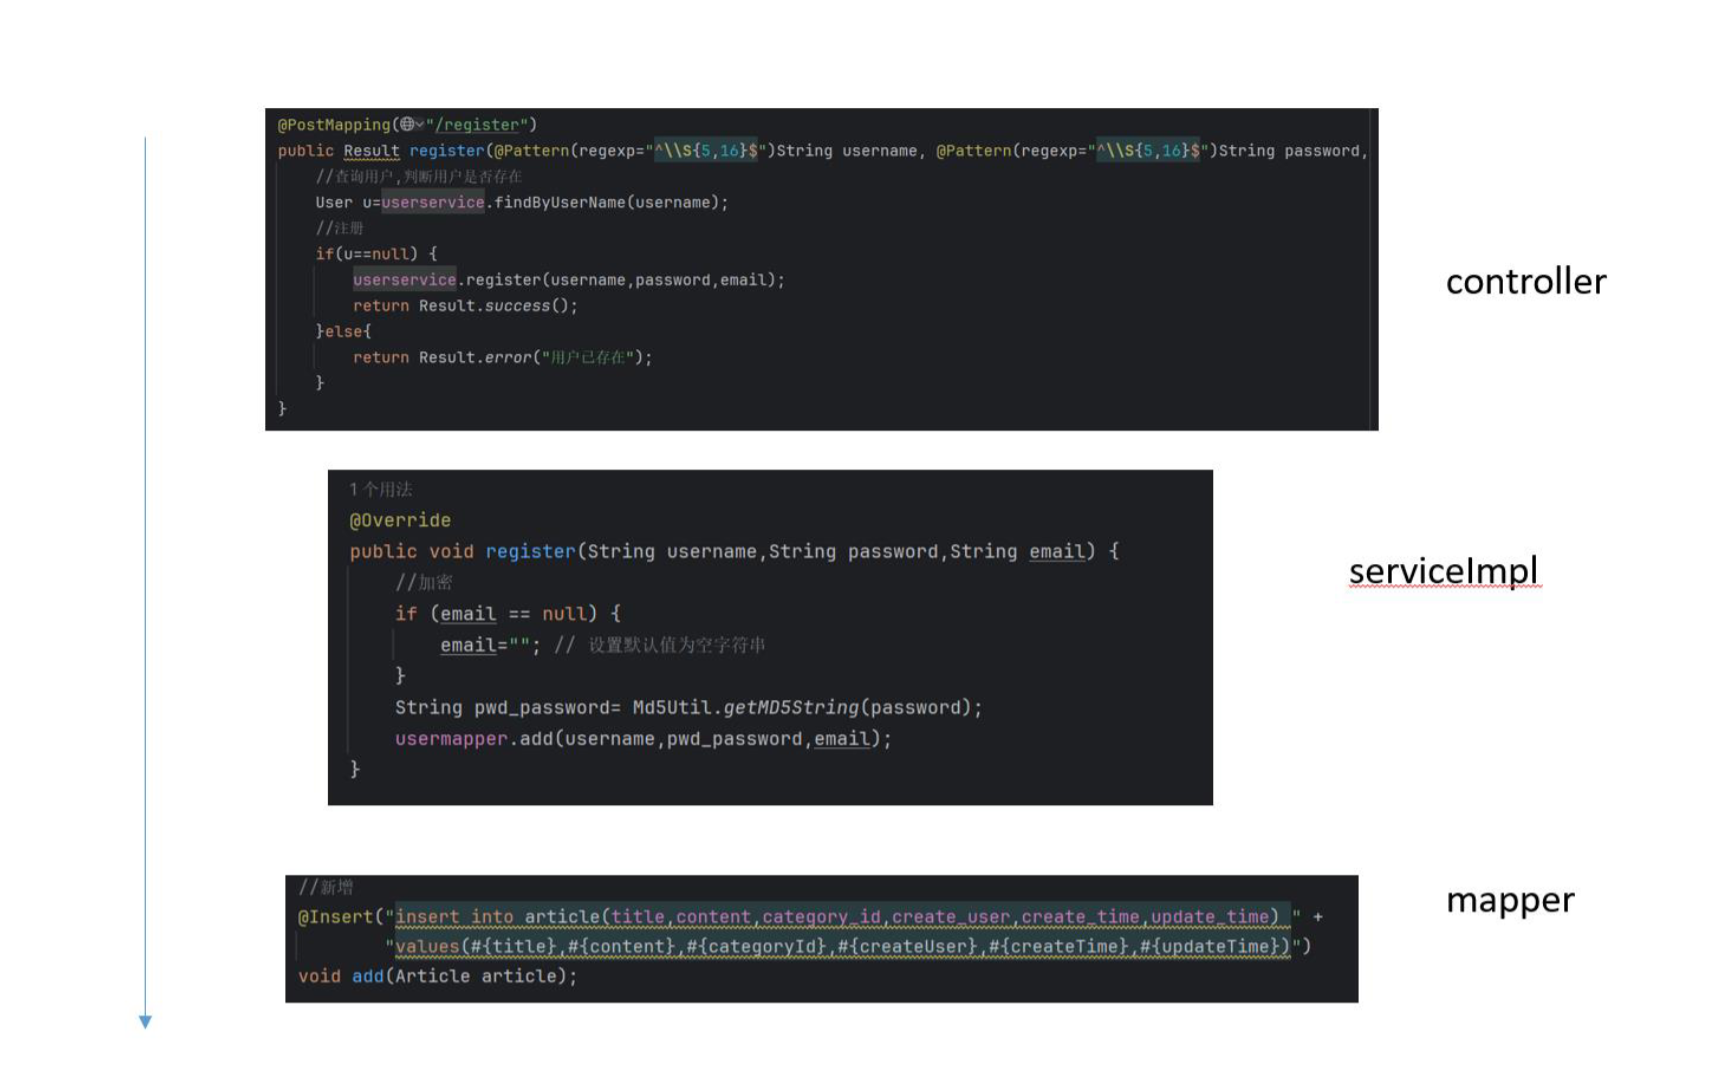
\includegraphics[width=1.0\textwidth]{register.png}
    \caption{注册}
    \label{re}
\end{figure}


\subsubsection{登录}
1.查询判断用户是否存在。
2.判断密码是否正确。
3.得到 jwt 令牌。
如图\ref{lo}所示。
\begin{figure}[htbp]
    \centering
    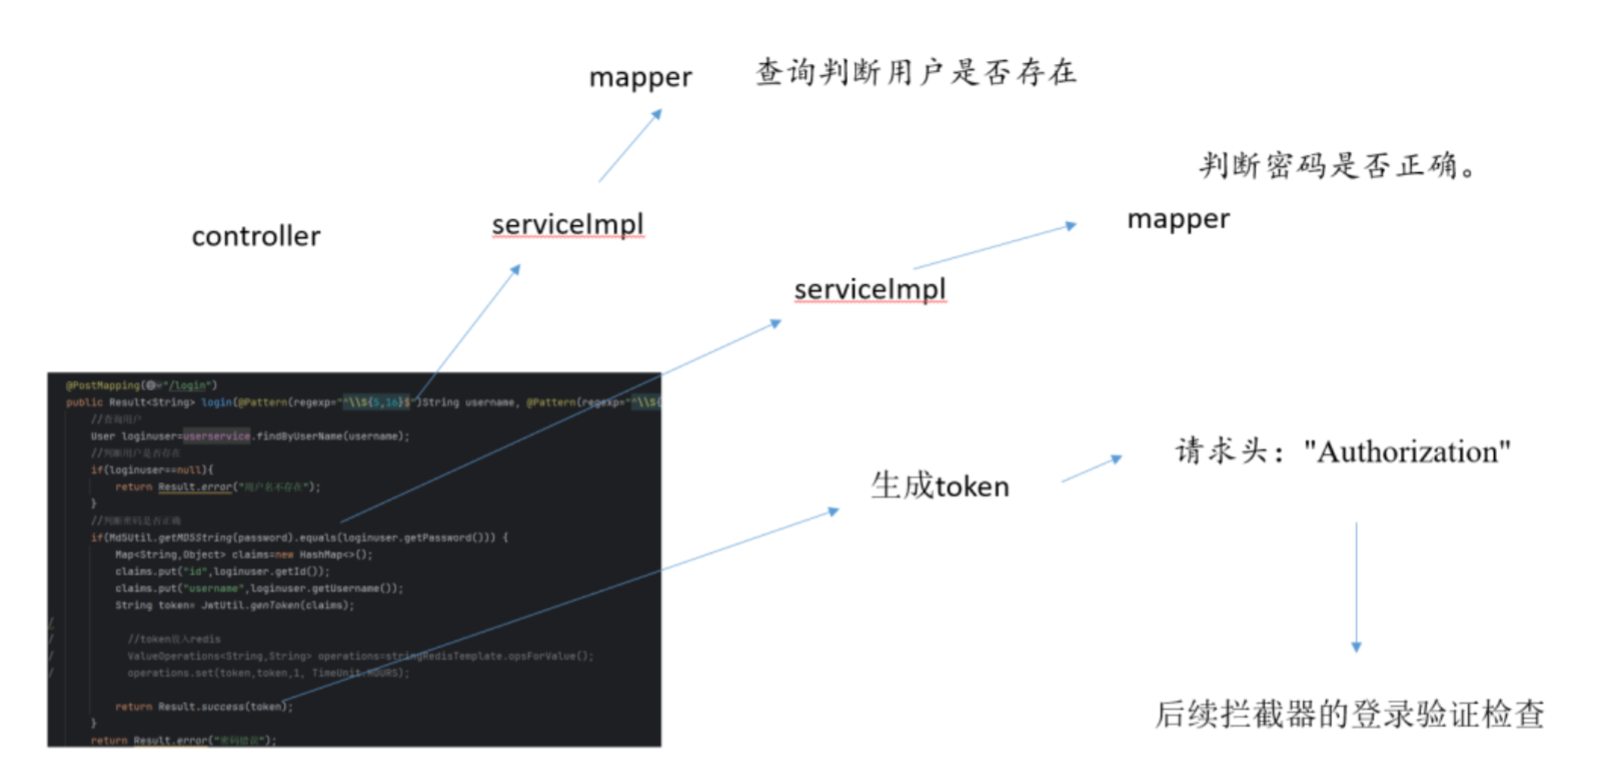
\includegraphics[width=1.0\textwidth]{login.png}
    \caption{登录}
    \label{lo}
\end{figure}

\subsubsection{拦截器}
其他页面在无令牌的情况并且没有被排除在拦截器以外的请求,不让访问,
因为其没有登录。
1.通过实现 WebMvcConfigurer 接口并重写 addInterceptors 方法,Spring MVC
能够使用自定义的拦截器来对请求进行处理。
2.LoginInterceptor 是 Spring MVC 中 HandlerInterceptor 接 口 的 实 现 类 。
HandlerInterceptor 是 Spring 提供的一种拦截器机制,允许你在请求的处理链中,
在控制器方法执行前、后或者完成时进行处理。具体来说,LoginInterceptor 作
为自定义的拦截器,用于处理登录验证的逻辑。
3.自定义的 LoginInterceptor,用于在请求到达控制器之前检查用户的登录状态。
具体来说,它通过解析请求头中的 Authorization 字段中的 JWT(JSON Web
Token)来验证用户是否登录。如果验证成功,会将用户信息存储在当前线程的
ThreadLocal 中,供后续使用。如果验证失败,则拦截请求并返回 401 错误。
如图\ref{fi}所示。
\begin{figure}[htbp]
    \centering
    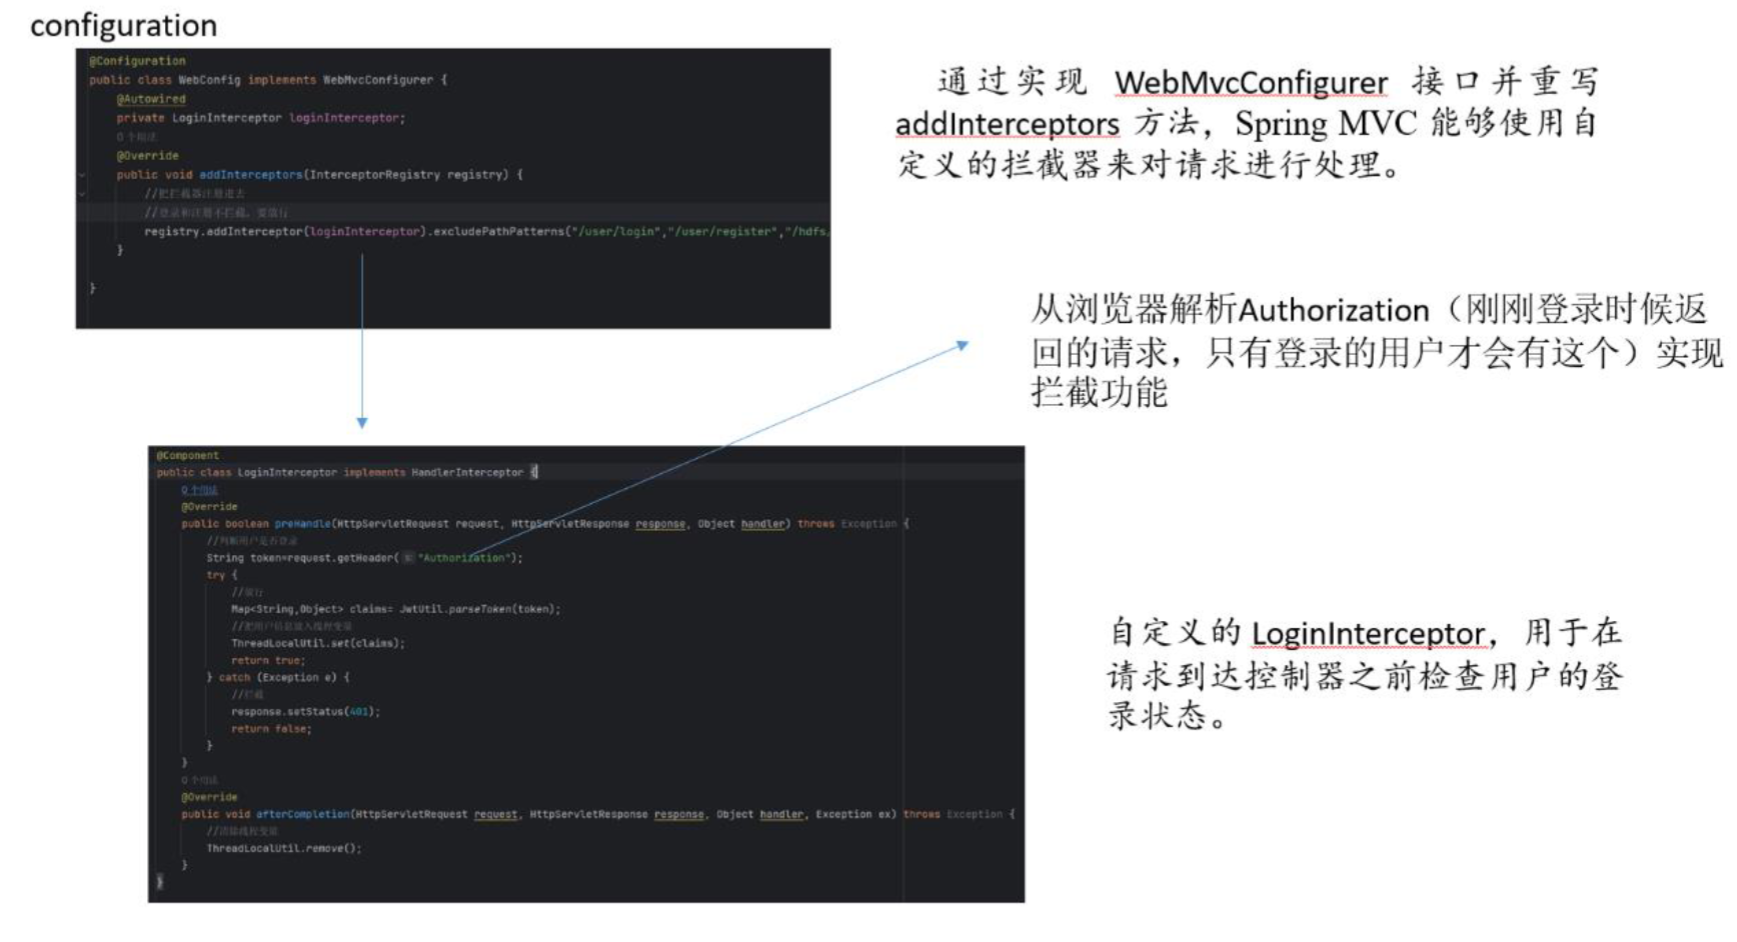
\includegraphics[width=1.0\textwidth]{filter.png}
    \caption{拦截器}
    \label{fi}
\end{figure}

\subsubsection{更新用户信息}
与之前的逻辑基本一致,不再赘述。
在这里补充我们在controller层用到的请求方法:
\begin{itemize}
\item 1. GET 请求
用途:用于从服务器获取资源。GET 请求是无副作用的,意味着它不会修
改任何数据,只是请求数据。
\item 2.POST 请求
用途:用于向服务器提交数据,通常用于创建新的资源。POST 请求会在服
务器上产生副作用,通常会创建、修改或触发某些操作。
\item 3. PUT 请求
用途:用于更新资源或创建资源。PUT 请求会覆盖指定的资源。如果资源
不存在,则可以创建该资源。
\item 4.DELETE 请求
用途:用于删除资源。DELETE 请求会删除服务器上的资源。
\end{itemize}
\subsection{文章功能}
\subsubsection{文章分类}
文章分类实现如图\ref{cate}所示,基本原理与用户注册登录类似,都是在通过分层设计实现。


\begin{figure}[htbp]
    \centering
    \subfloat[增加分类]{
        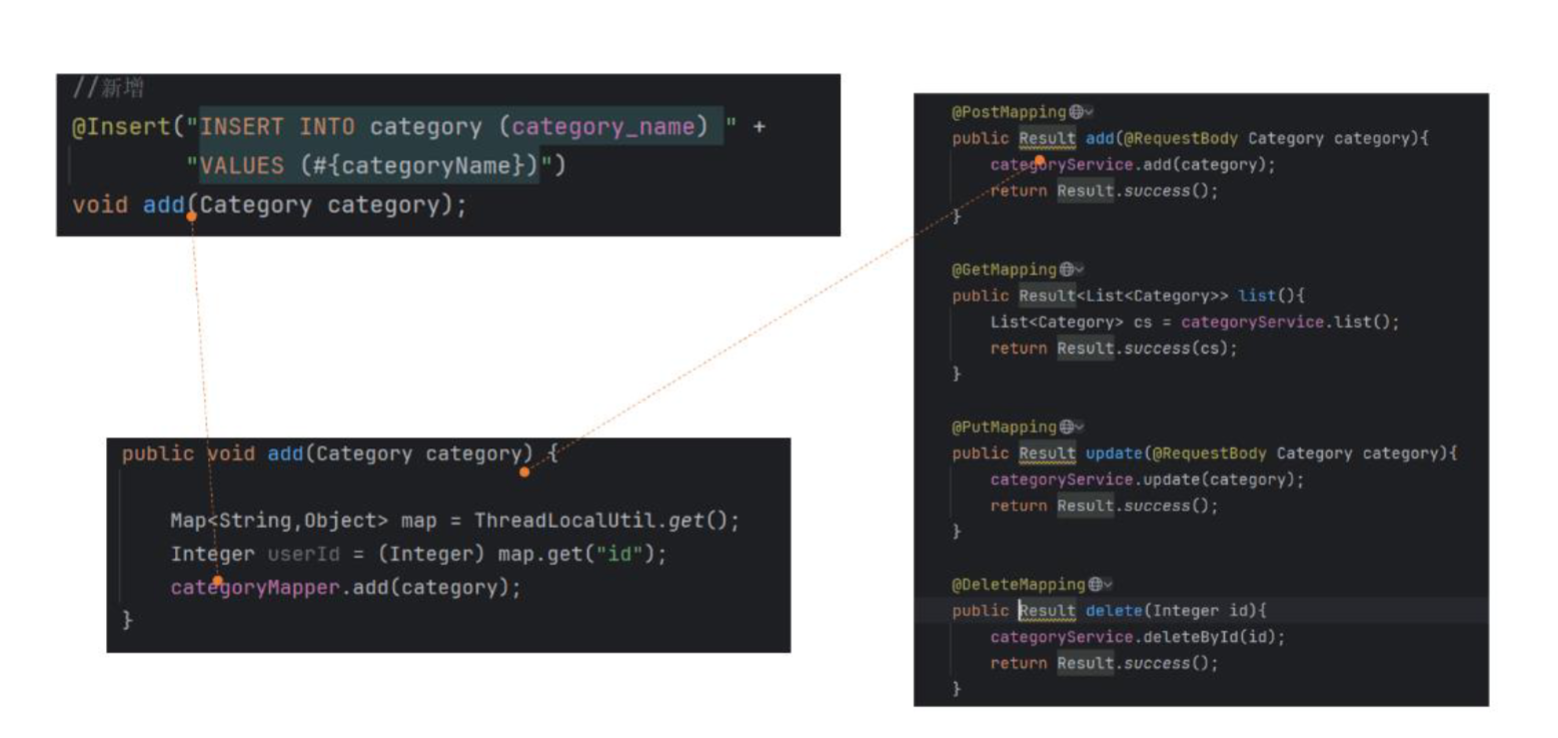
\includegraphics[width=0.45\textwidth]{cadd.png}
    }
    \subfloat[删除分类]{
        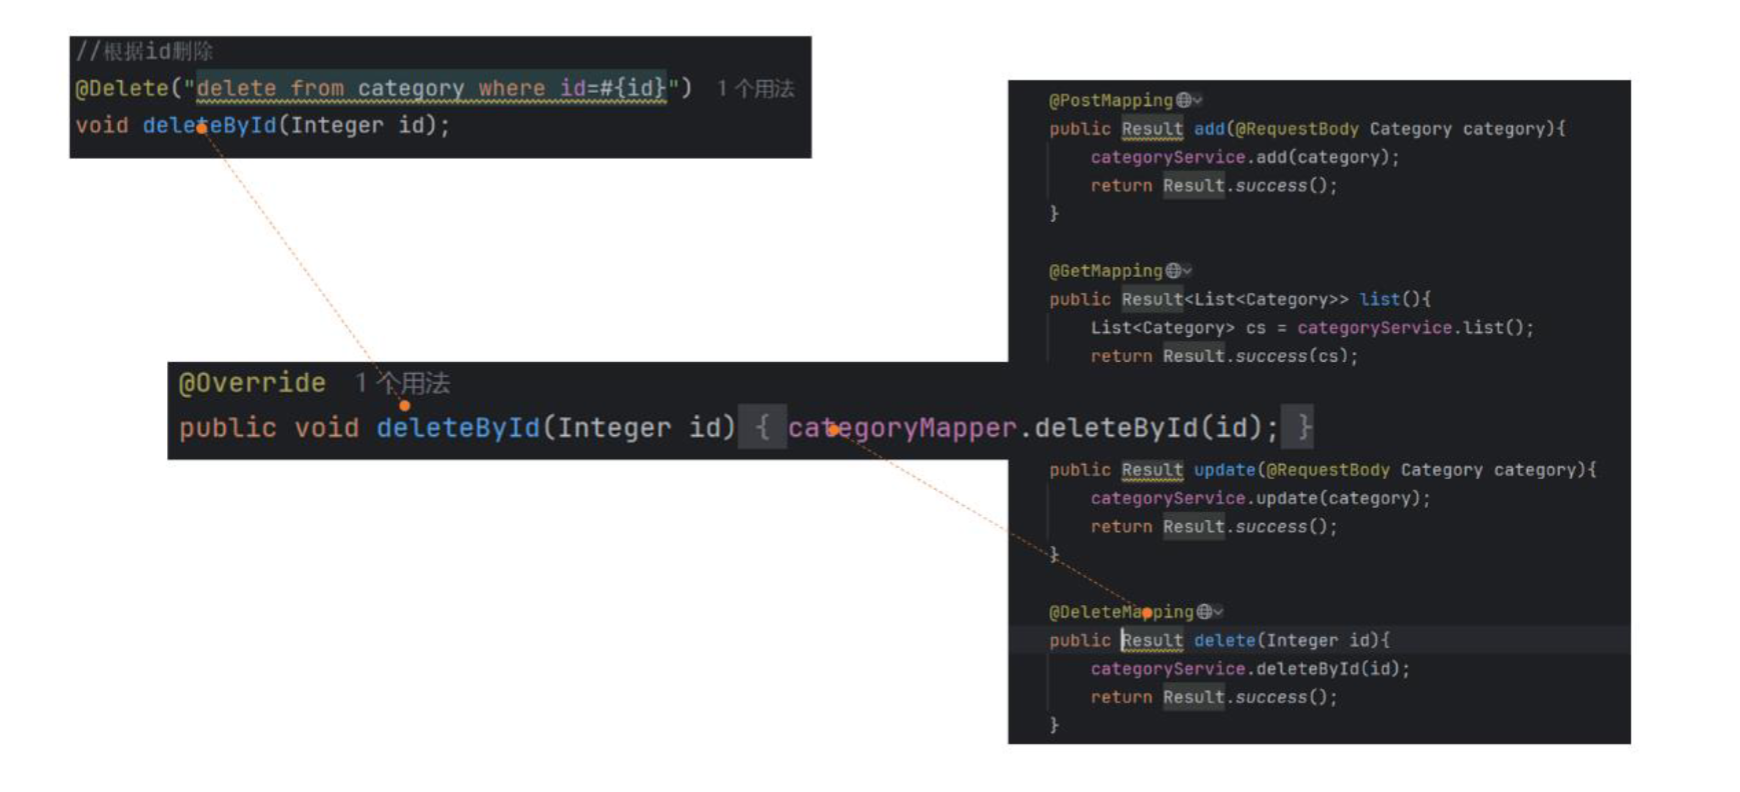
\includegraphics[width=0.45\textwidth]{cdel.png}
    }\\
    \subfloat[更新分类]{
        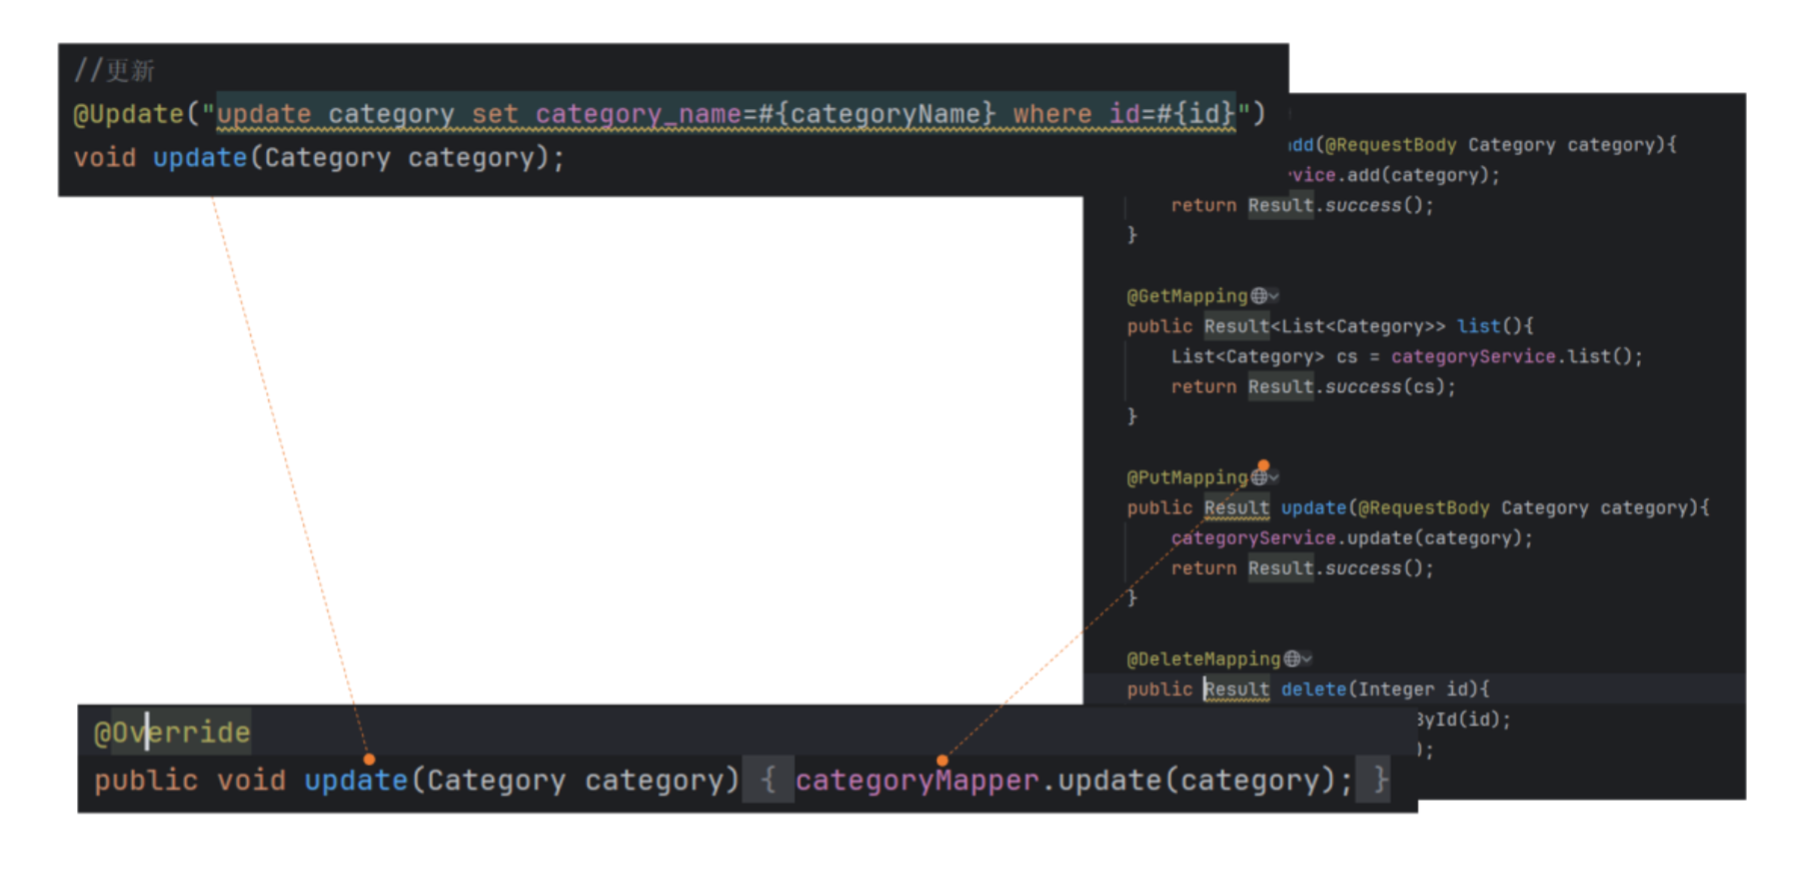
\includegraphics[width=0.45\textwidth]{cupdate.png}
    }
    \subfloat[查询分类]{
        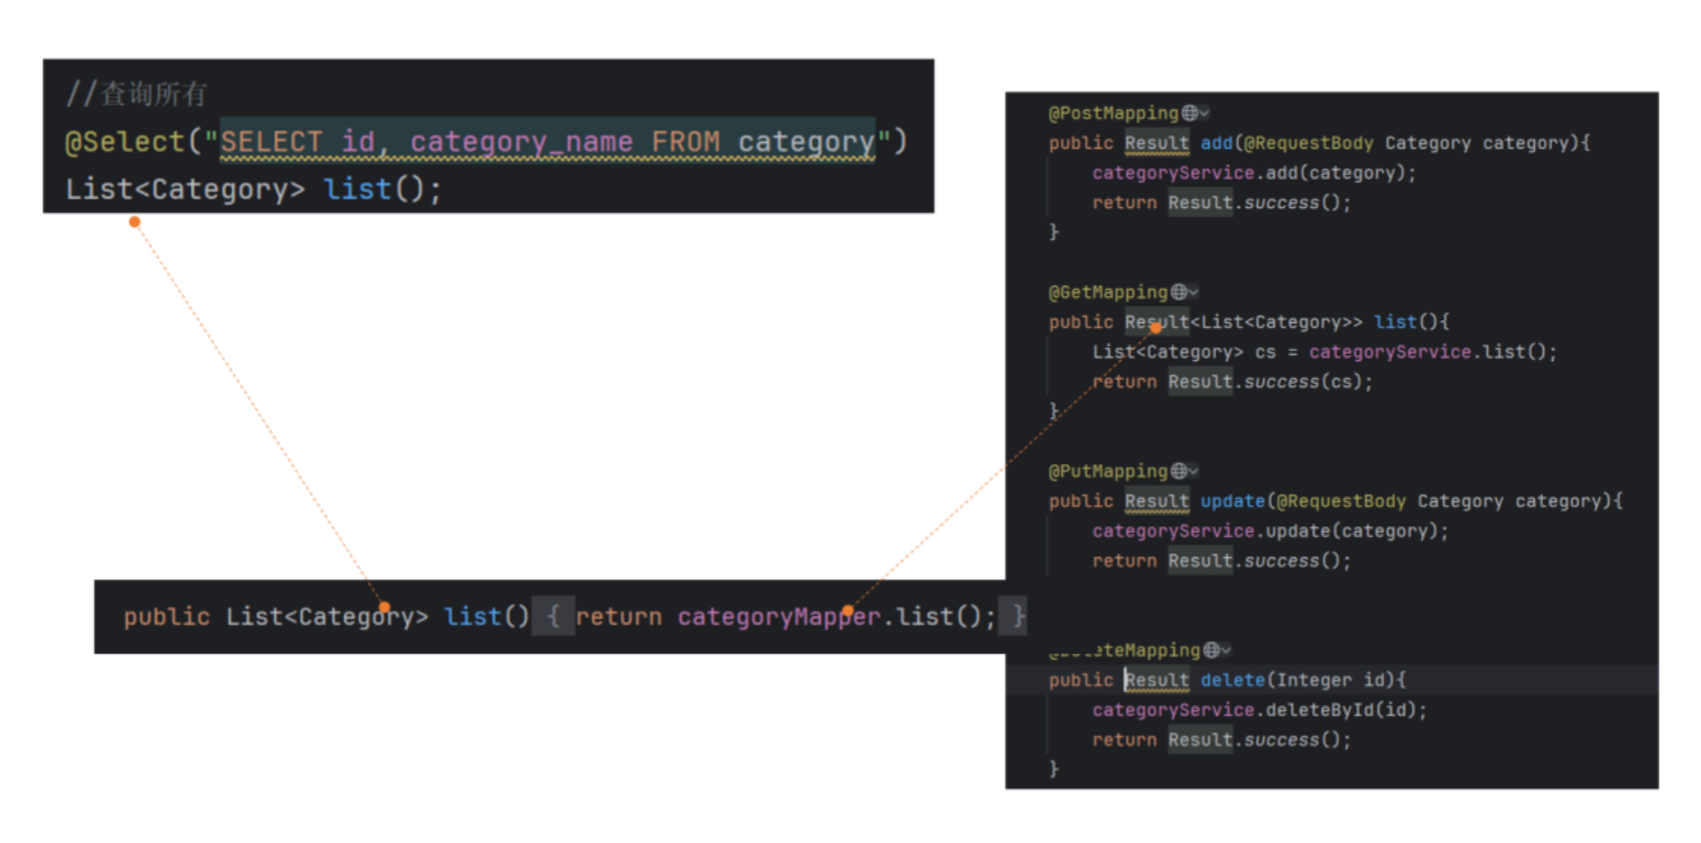
\includegraphics[width=0.45\textwidth]{cquery.png}
    }
    \caption{文章分类增删改查}
    \label{cate}
\end{figure}
\subsubsection{文章增删改查}
文章增删改查通过分层设计实现,主要代码如下:
\begin{itemize}
\item 1. 增加文章
\begin{lstlisting}[language=Java]
# controller
articleService.add(article);
# serviceImpl
if(articleMapper.fileExist(article.getTitle())){
    articleMapper.deleteById(article.getId());
}
articleMapper.add(article);
# 上传到hadoop
String[] paths=path(article);
String hadooppath=paths[0];
String rootpath=paths[1];
// 将 HTML 内容转为纯文本再上传
String plainText = Jsoup.parse(article.getContent()).text();
hadoopUtils.uploadArticleToHadoop(plainText, rootpath, hadooppath);
# mapper

void add(Article article);
@Select("SELECT COUNT(*)>0 FROM article WHERE title=#{filename}")
Boolean fileExist(String filename);
# hadoopUtils
// 先保存内容到本地文件,再上传到 HDFS(去重)
public void uploadArticleToHadoop(String content, String localPath, String hadoopPath) throws Exception {
    // 1. 保存内容到本地
    try (FileWriter writer = new FileWriter(localPath)) {
        writer.write(content);
    }

    // 2. 上传到 HDFS(去重)
    FileSystem fs = getFileSystem();
    Path hdfsPath = new Path(hadoopPath);
    try {
        if (fs.exists(hdfsPath)) {
            fs.delete(hdfsPath, true);
        }
        try (InputStream in = new FileInputStream(localPath);
                OutputStream out = fs.create(hdfsPath, true)) {
            IOUtils.copyBytes(in, out, 1024);
        }
    } finally {
        fs.close();
    }
}
\end{lstlisting}

\item 2. 分页展示文章
\begin{lstlisting}[language=Java]
# controller
PageBean<Article> pb =  articleService.list(pageNum,pageSize,categoryId,state);
# serviceImpl
//1.创建PageBean对象
PageBean<Article> pb = new PageBean<>();
//2.开启分页查询 PageHelper
PageHelper.startPage(pageNum, pageSize);
//3.调用mapper
Map<String, Object> map = ThreadLocalUtil.get();
Integer userId = (Integer) map.get("id");
List<Article> as = articleMapper.list();
//Page中提供了方法,可以获取PageHelper分页查询后 得到的总记录条数和当前页数据
Page<Article> p = (Page<Article>) as;
//把数据填充到PageBean对象中
pb.setTotal(p.getTotal());
pb.setItems(p.getResult());
return pb;
# mapper
@Select("SELECT * FROM article")
List<Article> list();
\end{lstlisting}



\item 3. 更新文章
\begin{lstlisting}[language=Java]
# controller
article a = articleService.update(article);
# serviceImpl
return articleMapper.update(article);
# mapper
Article update(Article article);
\end{lstlisting}


\item 4. 删除文章
\begin{lstlisting}[language=Java]
# controller
articleService.deleteById(id);
# serviceImpl
Article article=articleMapper.findById(id);
String[] paths=path(article);
String hadooppath=paths[0];
String rootpath=paths[1];
hadoopUtils.deleteFromHadoop(rootpath,hadooppath);
articleMapper.deleteById(id);
# mapper
@Delete("delete from article where id=#{id}")
void deleteById(Integer id);
@Select("select * FROM article where id=#{id}")
Article findById(Integer id);
# hadoopUtils
// 删除 HDFS 文件和本地文件
public void deleteFromHadoop(String localPath,String hadoopPath) throws Exception {
    FileSystem fs = getFileSystem();
    try {
        fs.delete(new Path(hadoopPath), true);
    } finally {
        fs.close();
    }
    java.io.File file = new java.io.File(localPath);
    if (file.exists()) {
        file.delete();
    }
}
\end{lstlisting}

\end{itemize}
\subsection{文件后端}
文件增加、删除、更新、查询、下载、预览等功能。(主要在controller层实现)
\begin{itemize}

\item 1. 文件上传
\begin{lstlisting}[language=Java]
@PostMapping(consumes = MediaType.MULTIPART_FORM_DATA_VALUE)
public ResponseEntity<FileInfo> uploadFile(
        @RequestParam("file") MultipartFile file) {  // 接收前端上传的Multipart文件
    try {
        // 1. 校验文件(例如大小、类型等,具体逻辑在validateFile方法中)
        validateFile(file);

        // 2. 确保上传目录存在(不存在则创建)
        Path uploadPath = Paths.get(uploadDir).toAbsolutePath().normalize();
        Files.createDirectories(uploadPath);

        // 3. 获取原始文件名并生成目标路径
        String originalFilename = Objects.requireNonNull(file.getOriginalFilename());
        Path targetPath = uploadPath.resolve(originalFilename);

        // 4. 保存文件到本地(覆盖同名文件)
        Files.copy(
            file.getInputStream(), 
            targetPath, 
            StandardCopyOption.REPLACE_EXISTING
        );
        System.out.println("文件上传成功,文件地址:" + targetPath);

        // 5. 上传文件到Hadoop(需替换为实际Hadoop工具类逻辑)
        String hadoopPath = hadoop + "/" + originalFilename;
        hadooputils.uploadFileToHadoop(targetPath.toString(), hadoopPath);

        // 6. 返回成功响应(包含文件名信息)
        return ResponseEntity.ok(new FileInfo(originalFilename));

    } catch (IllegalArgumentException e) {
        // 校验失败:返回400 Bad Request
        return ResponseEntity.badRequest().build();
    } catch (Exception e) {
        // 其他错误:返回500 Internal Server Error
        e.printStackTrace();  // 实际项目中建议用日志记录
        return ResponseEntity.internalServerError().build();
    }
}
\end{lstlisting}
\item 2. 文件展示与查询
\begin{lstlisting}[language=Java]
   @GetMapping
public ResponseEntity<Map<String, Object>> listFiles(
        @RequestParam(defaultValue = "1") int pageNum,      // 当前页码,默认为1
        @RequestParam(defaultValue = "5") int pageSize,    // 每页条数,默认为5
        @RequestParam(required = false) String filename)   // 可选文件名过滤条件
        throws IOException {
    
    // 1. 获取上传目录的绝对路径
    Path uploadPath = Paths.get(uploadDir).toAbsolutePath().normalize();
    Map<String, Object> result = new HashMap<>();
    
    // 2. 检查目录是否存在,若不存在返回空结果
    if (!Files.exists(uploadPath)) {
        result.put("items", Collections.emptyList());
        result.put("total", 0);
        return ResponseEntity.ok(result);
    }
    
    // 3. 遍历目录下的文件,过滤出符合条件的文件列表
    List<FileInfo> allFiles = Files.list(uploadPath)
            .filter(Files::isRegularFile)                  // 只保留普通文件(排除目录)
            .map(path -> new FileInfo(path.getFileName().toString())) // 转换为FileInfo对象
            .filter(info -> filename == null || filename.isEmpty() || 
                   info.getFilename().contains(filename)) // 按文件名模糊过滤
            .collect(Collectors.toList());
    
    // 4. 计算分页参数
    int total = allFiles.size();                           // 文件总数
    int fromIndex = Math.max(0, (pageNum - 1) * pageSize); // 当前页起始索引
    int toIndex = Math.min(fromIndex + pageSize, total);   // 当前页结束索引
    
    // 5. 截取分页数据(防止越界)
    List<FileInfo> pageList = fromIndex > total ? 
            Collections.emptyList() : 
            allFiles.subList(fromIndex, toIndex);
    
    // 6. 返回分页结果
    result.put("items", pageList);    // 当前页数据
    result.put("total", total);       // 总文件数
    return ResponseEntity.ok(result);
}
\end{lstlisting}
\item 3. 文件下载
\begin{lstlisting}[language=Java]
@GetMapping("/{filename}")
public void downloadFile(
        @PathVariable String filename,  // 从URL路径中获取文件名
        HttpServletResponse response)   // 直接操作HTTP响应流
        throws IOException {
    
    // 1. 构建文件绝对路径(安全处理)
    Path uploadPath = Paths.get(uploadDir).toAbsolutePath().normalize();
    Path filePath = uploadPath.resolve(filename);
    
    // 2. 检查文件是否存在
    if (!Files.exists(filePath)) {
        response.setStatus(HttpServletResponse.SC_NOT_FOUND); // 404
        return;
    }

    // 3. 处理文件名编码(解决中文/特殊字符问题)
    String encodedName = URLEncoder.encode(filename, StandardCharsets.UTF_8)
                                .replaceAll("\\+", "%20"); // 替换空格编码
    // 4. 自动探测MIME类型(失败时默认二进制流)
    String contentType = Files.probeContentType(filePath);
    if (contentType == null) {
        contentType = "application/octet-stream"; // 通用二进制类型
    }

    // 5. 设置响应头
    response.setContentType(contentType);
    response.setHeader("Content-Disposition", 
            "attachment; filename*=UTF-8''" + encodedName); // RFC 5987编码
    response.setHeader("Cache-Control", "no-cache, no-store, must-revalidate"); // 禁用缓存

    // 6. 流式传输文件内容
    try (InputStream is = Files.newInputStream(filePath);
         OutputStream os = response.getOutputStream()) {
        
        byte[] buffer = new byte[8192]; // 8KB缓冲区(平衡内存和IO效率)
        int len;
        while ((len = is.read(buffer)) != -1) {
            os.write(buffer, 0, len); // 分块写入响应流
        }
        os.flush();
        
    } catch (Exception e) {
        // 7. 处理传输异常
        response.setStatus(HttpServletResponse.SC_INTERNAL_SERVER_ERROR); // 500
        e.printStackTrace(); // 生产环境应替换为日志记录
    }
}
\end{lstlisting}
\item 4. 文件删除
\begin{lstlisting}[language=Java]
@DeleteMapping("/{filename}")
public ResponseEntity<Void> deleteFile(
        @PathVariable String filename) {  // 从URL路径获取待删除文件名
    
    // 1. 构建文件绝对路径(安全处理)
    Path uploadPath = Paths.get(uploadDir).toAbsolutePath().normalize();
    Path filePath = uploadPath.resolve(filename);

    try {
        // 2. 检查文件是否存在
        if (!Files.exists(filePath)) {
            return ResponseEntity.notFound().build(); // 404
        }

        // 3. 删除本地文件
        Files.delete(filePath); // 可能抛出IOException

        // 4. 同步删除Hadoop中的文件(假设hadooputils已实现)
        String hadoopPath = hadoop + "/" + filename;
        hadooputils.deleteFromHadoop(filePath.toString(), hadoopPath);

        // 5. 返回204 No Content(删除成功无返回值)
        return ResponseEntity.noContent().build();

    } catch (IOException e) {
        // 6. 文件操作异常(如权限不足、磁盘错误)
        return ResponseEntity.internalServerError().build(); // 500
    } catch (Exception e) {
        // 7. 其他未知异常(如Hadoop连接失败)
        throw new RuntimeException("文件删除失败", e); // 转换为非受检异常
    }
}
\end{lstlisting}

\item 5. 文件预览
\begin{lstlisting}[language=Java]
@GetMapping("/preview/{filename}")
public void previewFile(
        @PathVariable String filename,  // 从URL路径获取文件名
        HttpServletResponse response)   // 直接操作HTTP响应流
        throws IOException {
    
    // 1. 构建文件绝对路径(安全处理)
    Path uploadPath = Paths.get(uploadDir).toAbsolutePath().normalize();
    Path filePath = uploadPath.resolve(filename);

    // 2. 检查文件是否存在
    if (!Files.exists(filePath)) {
        response.setStatus(HttpServletResponse.SC_NOT_FOUND); // 404
        return;
    }

    // 3. 自动探测MIME类型(失败时默认二进制流)
    String contentType = Files.probeContentType(filePath);
    if (contentType == null) {
        contentType = "application/octet-stream"; // 通用二进制类型
    }

    // 4. 设置响应头(与下载接口的区别:无Content-Disposition头)
    response.setContentType(contentType);
    response.setHeader("Cache-Control", "no-cache, no-store, must-revalidate"); // 禁用缓存

    // 5. 流式传输文件内容
    try (InputStream is = Files.newInputStream(filePath);
         OutputStream os = response.getOutputStream()) {
        
        byte[] buffer = new byte[8192]; // 8KB缓冲区
        int len;
        while ((len = is.read(buffer)) != -1) {
            os.write(buffer, 0, len); // 分块写入响应流
        }
        os.flush();
        
    } catch (IOException e) {
        // 6. 处理传输异常(生产环境应记录日志)
        response.setStatus(HttpServletResponse.SC_INTERNAL_SERVER_ERROR); // 500
        e.printStackTrace(); // 替换为日志记录,如log.error("文件传输中断", e);
    }
}
\end{lstlisting}
\end{itemize}

\subsection{WordCount作业}
作业整体架构如图\ref{mrs1}所示,主要分为 Mapper、Reducer、Driver 三个部分。代码结构如图\ref{mrs2}所示,分为dowork与show。
\begin{figure}[htbp]
    \centering
    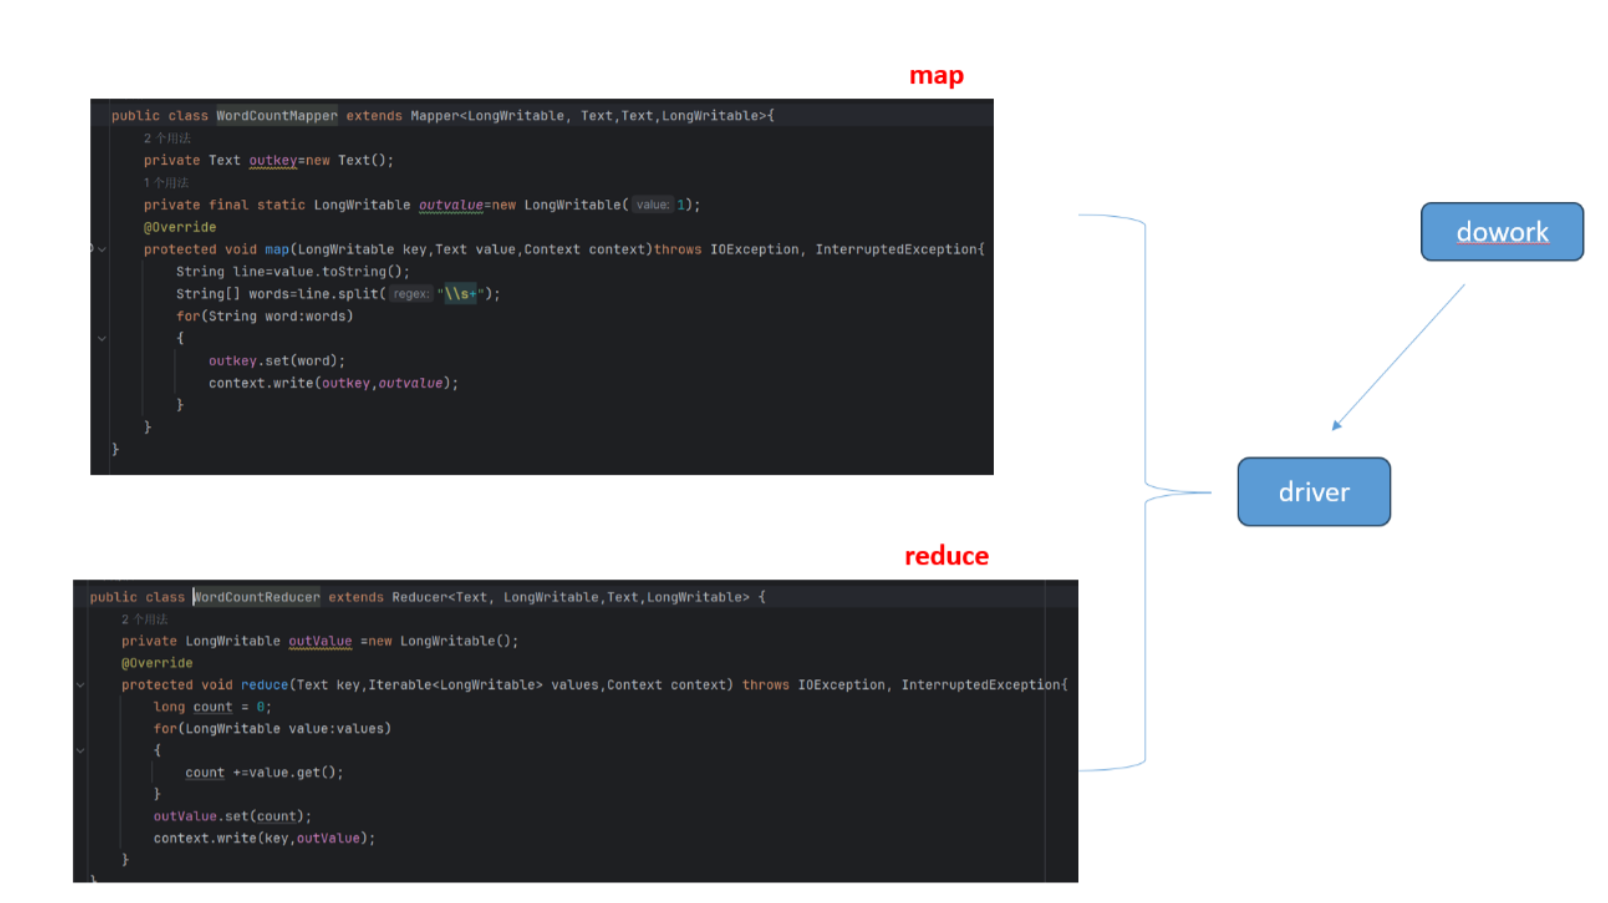
\includegraphics[width=0.7\textwidth]{mr_see.png}
    \caption{WordCount架构}
    \label{mrs1}
\end{figure}
\begin{figure}[htbp]
    \centering
    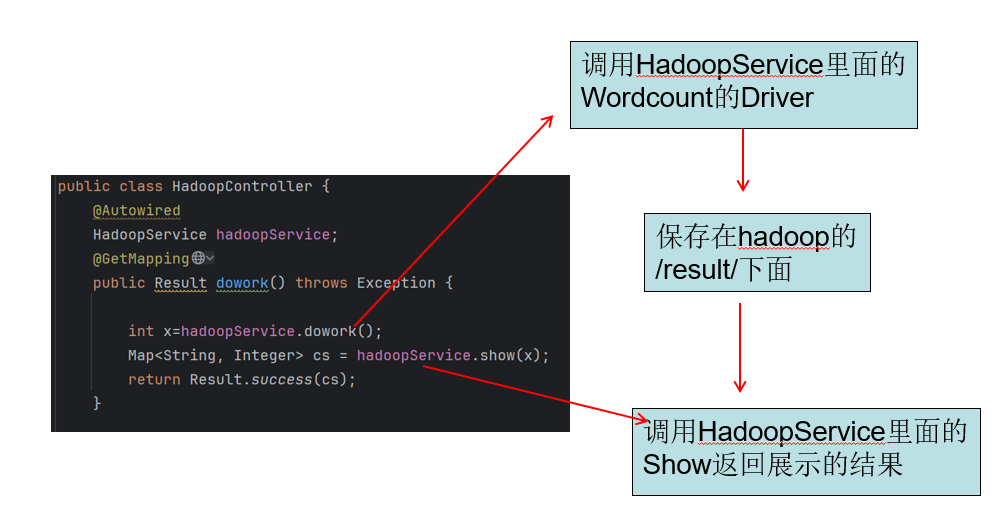
\includegraphics[width=0.7\textwidth]{mr_see2.png}
    \caption{WordCount作业}
    \label{mrs2}
\end{figure}


\section{前端搭建}
\subsection{前端框架}
如图\ref{vue1}所示。
api/: 封装所有后端HTTP请求;
assets/: 静态资源(如图片、样式);
router:定义应用的路由映射关系,路径到组件的映射(如/login → LoginView.vue);
stores:作用:集中管理跨组件共享的状态,例如记录用户登录状态(token);
utils: 工具函数;
view: 视图组件;
App.vue:应用的根组件,用于全局布局(如导航栏、页脚),<RouterView>用于显示当前路由匹配的页面组件;
main.js作用:Vue应用的启动入口,关键操作:初始化Vue实例并挂载到index.html的\#app节点,注册全局依赖(路由Router、状态管理Pinia);
index.html:应用的HTML骨架,Vue组件最终会渲染到\#app容器中。

\begin{figure}[htbp]
    \centering
    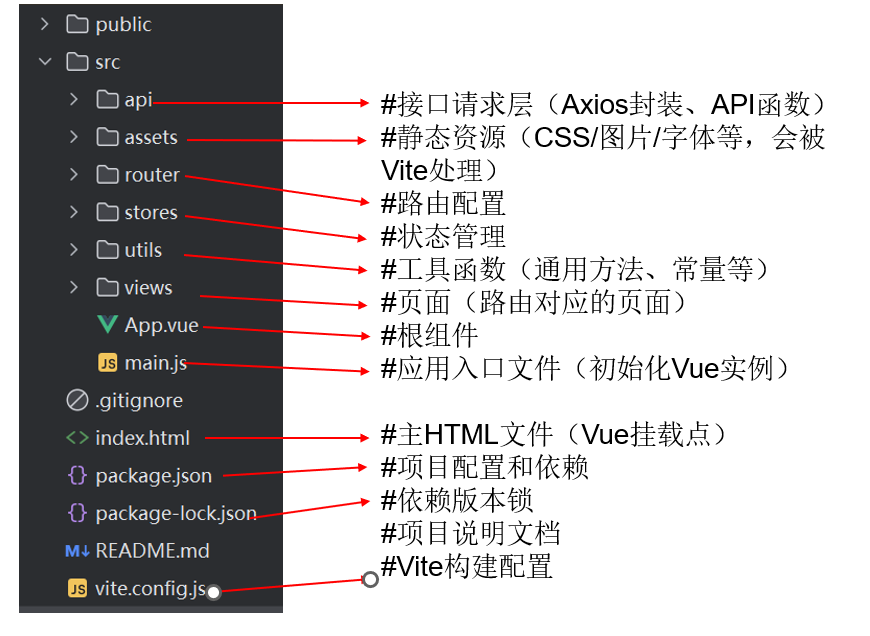
\includegraphics[width=0.7\textwidth]{vue_1.png}
    \caption{vue框架}
    \label{vue1}
\end{figure}

\subsection{拦截器与响应器}
请求拦截器:\\
动态从Pinia(tokenStore)获取Token,并自动附加到请求头。
避免手动在每个请求中重复设置Token,提高代码复用性。\\
响应拦截器:\\
业务数据提取:普通API请求直接返回response.data,减少冗余代码。
文件下载兼容:对responseType: 'blob的请求保留完整响应,确保能读取文件流和响应头(如文件名)。
统一错误处理:拦截401状态码,自动跳转登录页并提示用户,增强安全性。
\begin{lstlisting}
// 请求拦截器
instance.interceptors.request.use(
    config => {
        const tokenStore = useTokenStore()
        if (tokenStore.token) {
            config.headers.Authorization = tokenStore.token
        }
        return config
    },
    err => Promise.reject(err)
)
// 响应拦截器
instance.interceptors.response.use(
    response => {
        // 关键:下载接口返回完整 response
        if (response.config.responseType === 'blob') {
            return response
        }
        // 只处理 HTTP 层面,业务错误不 reject
        return response.data
    },
    err => {
        if (err.response && err.response.status === 401) {
            ElMessage.error('请先登录')
            router.push('/login')
        }
        return Promise.reject(err)
    }
)
\end{istlisting}

\subsection{路由配置}

\begin{lstlisting}[language=javascript]
    //定义路由关系
const routes = [
    { path: '/login', component: LoginVue },
    {
        path: '/', component: LayoutVue,redirect:'/article/manage', children: [
            { path: '/article/category', component: ArticleCategoryVue },
            { path: '/article/manage', component: ArticleManageVue },
            {path:'/article/hadoop',component: ArticleHadoop},
            { path: '/user/info', component: UserInfoVue },
            { path: '/user/resetPassword', component: UserResetPasswordVue },
            { path: '/file',name: '/file',component: FileViewVue},
        ],

    },


]

//创建路由器
const router = createRouter({
    history: createWebHistory(),
    routes: routes
})

//导出路由
export default router

\end{lstlisting}


\subsection{登录注册页面}
\begin{itemize}
\item 脚本部分:
引入 Element Plus 图标、消息提示、表单等组件。
使用 ref 定义响应式变量,如 isRegister 控制注册/登录表单切换,registerData 存储表单数据。
定义表单校验规则和自定义校验函数(如确认密码一致性)。
引入并调用后端接口(userRegisterService、userLoginService)实现注册和登录功能,登录成功后将 token 存储到 pinia,并跳转首页
\\关键代码:
\begin{lstlisting}
// 控制注册与登录表单显示
const isRegister = ref(false)
// 数据模型
const registerData = ref({
    username: '',
    password: '',
    rePassword: ''
})
// 注册
const register = async () => {
    let result = await userRegisterService(registerData.value)
    ElMessage.success(result.msg ? result.msg : '注册成功')
}
// 登录
const login = async () => {
    let result = await userLoginService(registerData.value)
    ElMessage.success(result.msg ? result.msg : '登录成功')
    tokenStore.setToken(result.data)
    router.push('/')
}
// 切换表单并清空数据
const clearRegisterData = () => {
    registerData.value = { username: '', password: '', rePassword: '' }
}
\end{lstlisting}

\item 模板部分:
根据 isRegister显示注册或登录表单,表单内包含用户名、密码、确认密码输入框及相关按钮。
注册/登录按钮绑定对应事件,底部有切换表单的链接。
定义CSS样式,设置表单布局、按钮样式等。
\\关键代码:
\begin{lstlisting}[language=html]
<!-- 表单切换与按钮绑定 -->
<el-card v-if="isRegister"> <!-- 注册表单 -->
  <el-button @click="register">注册</el-button>
  <el-link @click="isRegister = false;clearRegisterData()">← 返回</el-link>
</el-card>
<el-card v-else> <!-- 登录表单 -->
  <el-button @click="login">登录</el-button>
  <el-link @click="isRegister = true;clearRegisterData()">注册 →</el-link>
</el-card>
\end{lstlisting}
\item api部分:
\begin{lstlisting}
//导入request.js请求工具
import request from '@/utils/request.js'
//提供调用注册接口的函数
export const userRegisterService = (registerData)=>{
    //借助于UrlSearchParams完成传递
    const params = new URLSearchParams()
    for(let key in registerData){
        params.append(key,registerData[key]);
    }
    return request.post('/user/register',params);
}
//提供调用登录接口的函数
export const userLoginService = (loginData)=>{
    const params = new URLSearchParams();
    for(let key in loginData){
        params.append(key,loginData[key])
    }
    return request.post('/user/login',params)
}
//获取用户详细信息
export const userInfoService = ()=>{
    return request.get('/user/userInfo')
}
//修改个人信息
export const userInfoUpdateService = (userInfoData)=>{
   return request.put('/user/update',userInfoData)
}
export const updatePasswordService = (passwordData, token) => {
    return request.patch('/user/updatePwd', passwordData, {
        headers: {
            'Authorization': `Bearer ${token}`
        }
    });
};
\end{lstlisting}
\end{itemize}

\subsection{文章管理页面}

\begin{itemize}
\item 脚本部分:
引入表格、分页、弹窗等 Element Plus 组件。
定义文章列表数据、分页参数、查询条件(如分类、状态)。
提供获取文章列表、删除文章、跳转编辑等方法。
\\关键代码:
\begin{lstlisting}
const addArticle = async ()=>{
    //调用接口
    let result = await articleAddService(articleModel.value);
    ElMessage.success(result.msg? result.msg:'添加成功');

    //让抽屉消失
    visibleDrawer.value = false;

    //刷新当前列表
    articleList()
}
const showArticle = (row)=>{
    //显示抽屉
    visibleDrawer.value = true;
    //数据拷贝
    articleModel.value.title = row.title;
    articleModel.value.categoryId = row.categoryId;
    articleModel.value.content = row.content;
    articleModel.value.id = row.id;
}
\end{lstlisting}

\item 模板部分:
顶部为筛选表单(分类、状态、搜索)。
中间为文章数据表格,展示标题、分类、作者、状态、操作(编辑/删除)。
底部为分页组件。

\item api部分:
\begin{lstlisting}
import request from '@/utils/request.js'
import { useTokenStore } from '@/stores/token.js'
//文章分类列表查询
export const articleCategoryListService = ()=>{
    //const tokenStore = useTokenStore();
    //在pinia中定义的响应式数据,都不需要.value
    //return request.get('/category',{headers:{'Authorization':tokenStore.token}})
    return request.get('/category')
}

//文章分类添加
export const articleCategoryAddService = (categoryData)=>{
    return request.post('/category',categoryData)
}

//文章分类修改
export const articleCategoryUpdateService = (categoryData)=>{
   return  request.put('/category',categoryData)
}

//文章分类删除
export const articleCategoryDeleteService = (id)=>{
    return request.delete('/category?id='+id)
}

//文章列表查询
export const articleListService = (params)=>{
   return  request.get('/article',{params:params})
}

//文章添加
export const articleAddService = (articleData)=>{
    return request.post('/article',articleData);

}
export const articleUpdateService = (articleData)=>{
    return request.put('/article',articleData)
}
export const articleDeleteService = (id)=>{
    return request.delete('/article?id='+id)
}
export const articleupdataService = (articleData)=>{
    return request.put('/article',articleData)
}
export const hadoopList=()=>{
    return request.get('/hadoop');
}
\end{lstlisting}
\end{itemize}


\subsection{文件页面}

\begin{itemize}
\item 脚本部分:
主要用于文件的上传、下载、删除、预览和分页管理
\begin{lstlisting}
// 文件列表获取
const fetchFiles = async () => {
  const res = await fileListService({
    pageNum: pageNum.value,
    pageSize: pageSize.value,
    filename: searchName.value
  })
  files.value = res?.items || []
  total.value = res?.total || 0
}

// 文件上传
const uploadFile = async (option) => {
  const formData = new FormData()
  formData.append('file', option.file)
  await fileUploadService(formData)
  ElMessage.success('上传成功')
  fetchFiles()
}

// 文件下载
const downloadFile = async (filename) => {
  const response = await fileDownloadService(filename)
  const blob = response.data || response
  const url = window.URL.createObjectURL(blob)
  const link = document.createElement('a')
  link.href = url
  link.setAttribute('download', filename)
  document.body.appendChild(link)
  link.click()
  link.remove()
  window.URL.revokeObjectURL(url)
}

// 文件删除
const deleteFile = (row) => {
  ElMessageBox.confirm('你确认要删除该文件吗?', '温馨提示')
    .then(async () => {
      await fileDeleteService(row.filename)
      ElMessage.success('删除成功')
      fetchFiles()
    })
}

// 文件预览
const previewFile = async (filename) => {
  const response = await filePreviewService(filename)
  const blob = response.data || response
  previewUrl.value = window.URL.createObjectURL(blob)
  // 根据文件类型设置预览方式
  // ...
  previewVisible.value = true
}
\end{lstlisting}

\item 模板部分:
基本和上述一致。
\item api部分:
\begin{lstlisting}
import request from '@/utils/request.js'

export const fileListService = (params) => {
    return request.get('/api/files', { params })
}

export const fileUploadService = (formData) => {
    return request.post('/api/files', formData, {
        headers: { 'Content-Type': 'multipart/form-data' }
    })
}

export const fileDeleteService = (filename) => {
    return request.delete(`/api/files/${filename}`)
}

// 正确导出下载服务
export const fileDownloadService = (filename) => {
    return request({
        url: `/api/files/${encodeURIComponent(filename)}`,
        method: 'GET',
        responseType: 'blob'
    })
}

// src/api/file.js
export const filePreviewService = (filename) => {
    return request({
        url: `/api/files/preview/${encodeURIComponent(filename)}`,
        method: 'GET',
        responseType: 'blob'
    })
}
\end{lstlisting}
\end{itemize}

\chapter{测试}
\section{注册登录测试}
\subsection{拦截器测试}
访问:http://localhost:5173/article/manage时,由于没有登录,拦截器会拦截请求并返回401错误,
如图\ref{l1}所示,并跳转到界面:
http://localhost:5173/login
\begin{figure}[htbp]
    \centering
    
\includegraphics[width=0.5\textwidth]{拦截器测试.png}
    \caption{拦截器测试}
    \label{l1}
\end{figure}
\subsection{注册测试}
如图\ref{rc1},\ref{rc2}所示。
\begin{figure}[htbp]
    \centering
    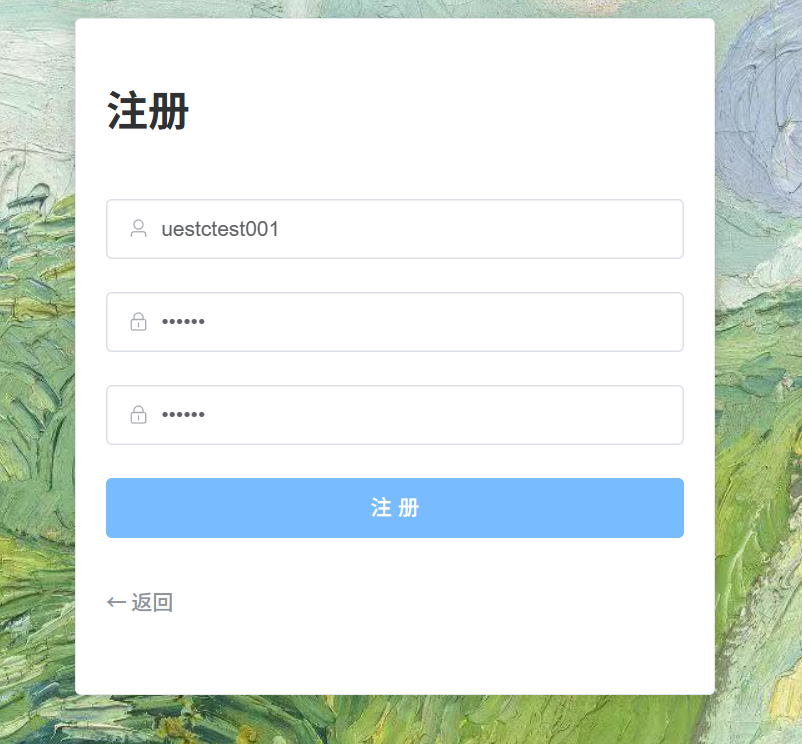
\includegraphics[width=0.5\textwidth]{注册1.png}
    \caption{注册界面}
    \label{rc1}
\end{figure}
\begin{figure}[htbp]
    \centering
    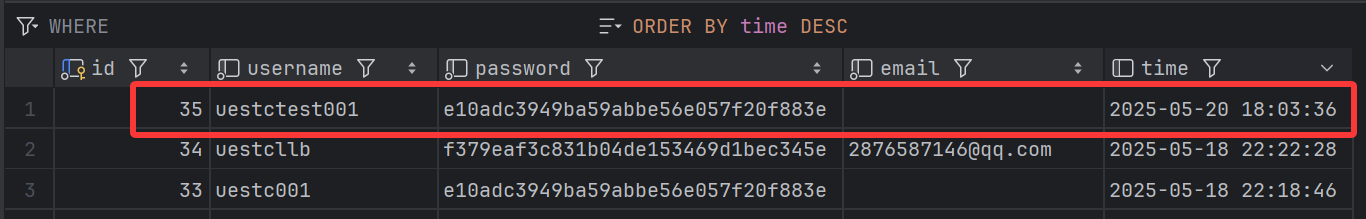
\includegraphics[width=0.5\textwidth]{注册2.png}
    \caption{后端数据库数据}
    \label{rc2}
\end{figure}
\subsection{登录测试}
登录界面:
如图\ref{dc2},\ref{dc3}所示。
\begin{figure}[htbp]
    \centering
    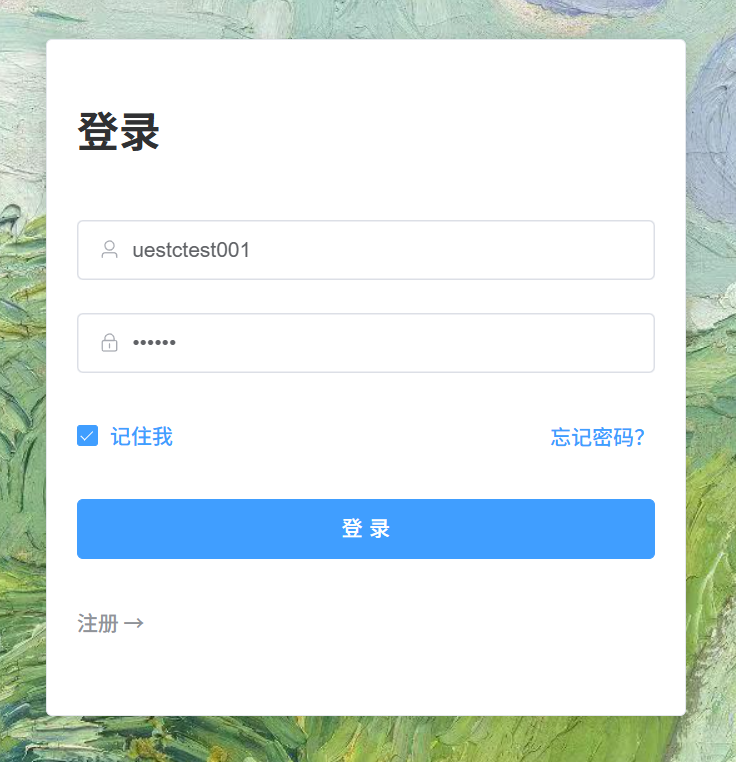
\includegraphics[width=0.5\textwidth]{登录.png}
    \caption{登录}
    \label{dc2}
\end{figure}
登录后的主界面:
\begin{figure}[htbp]
    \centering
    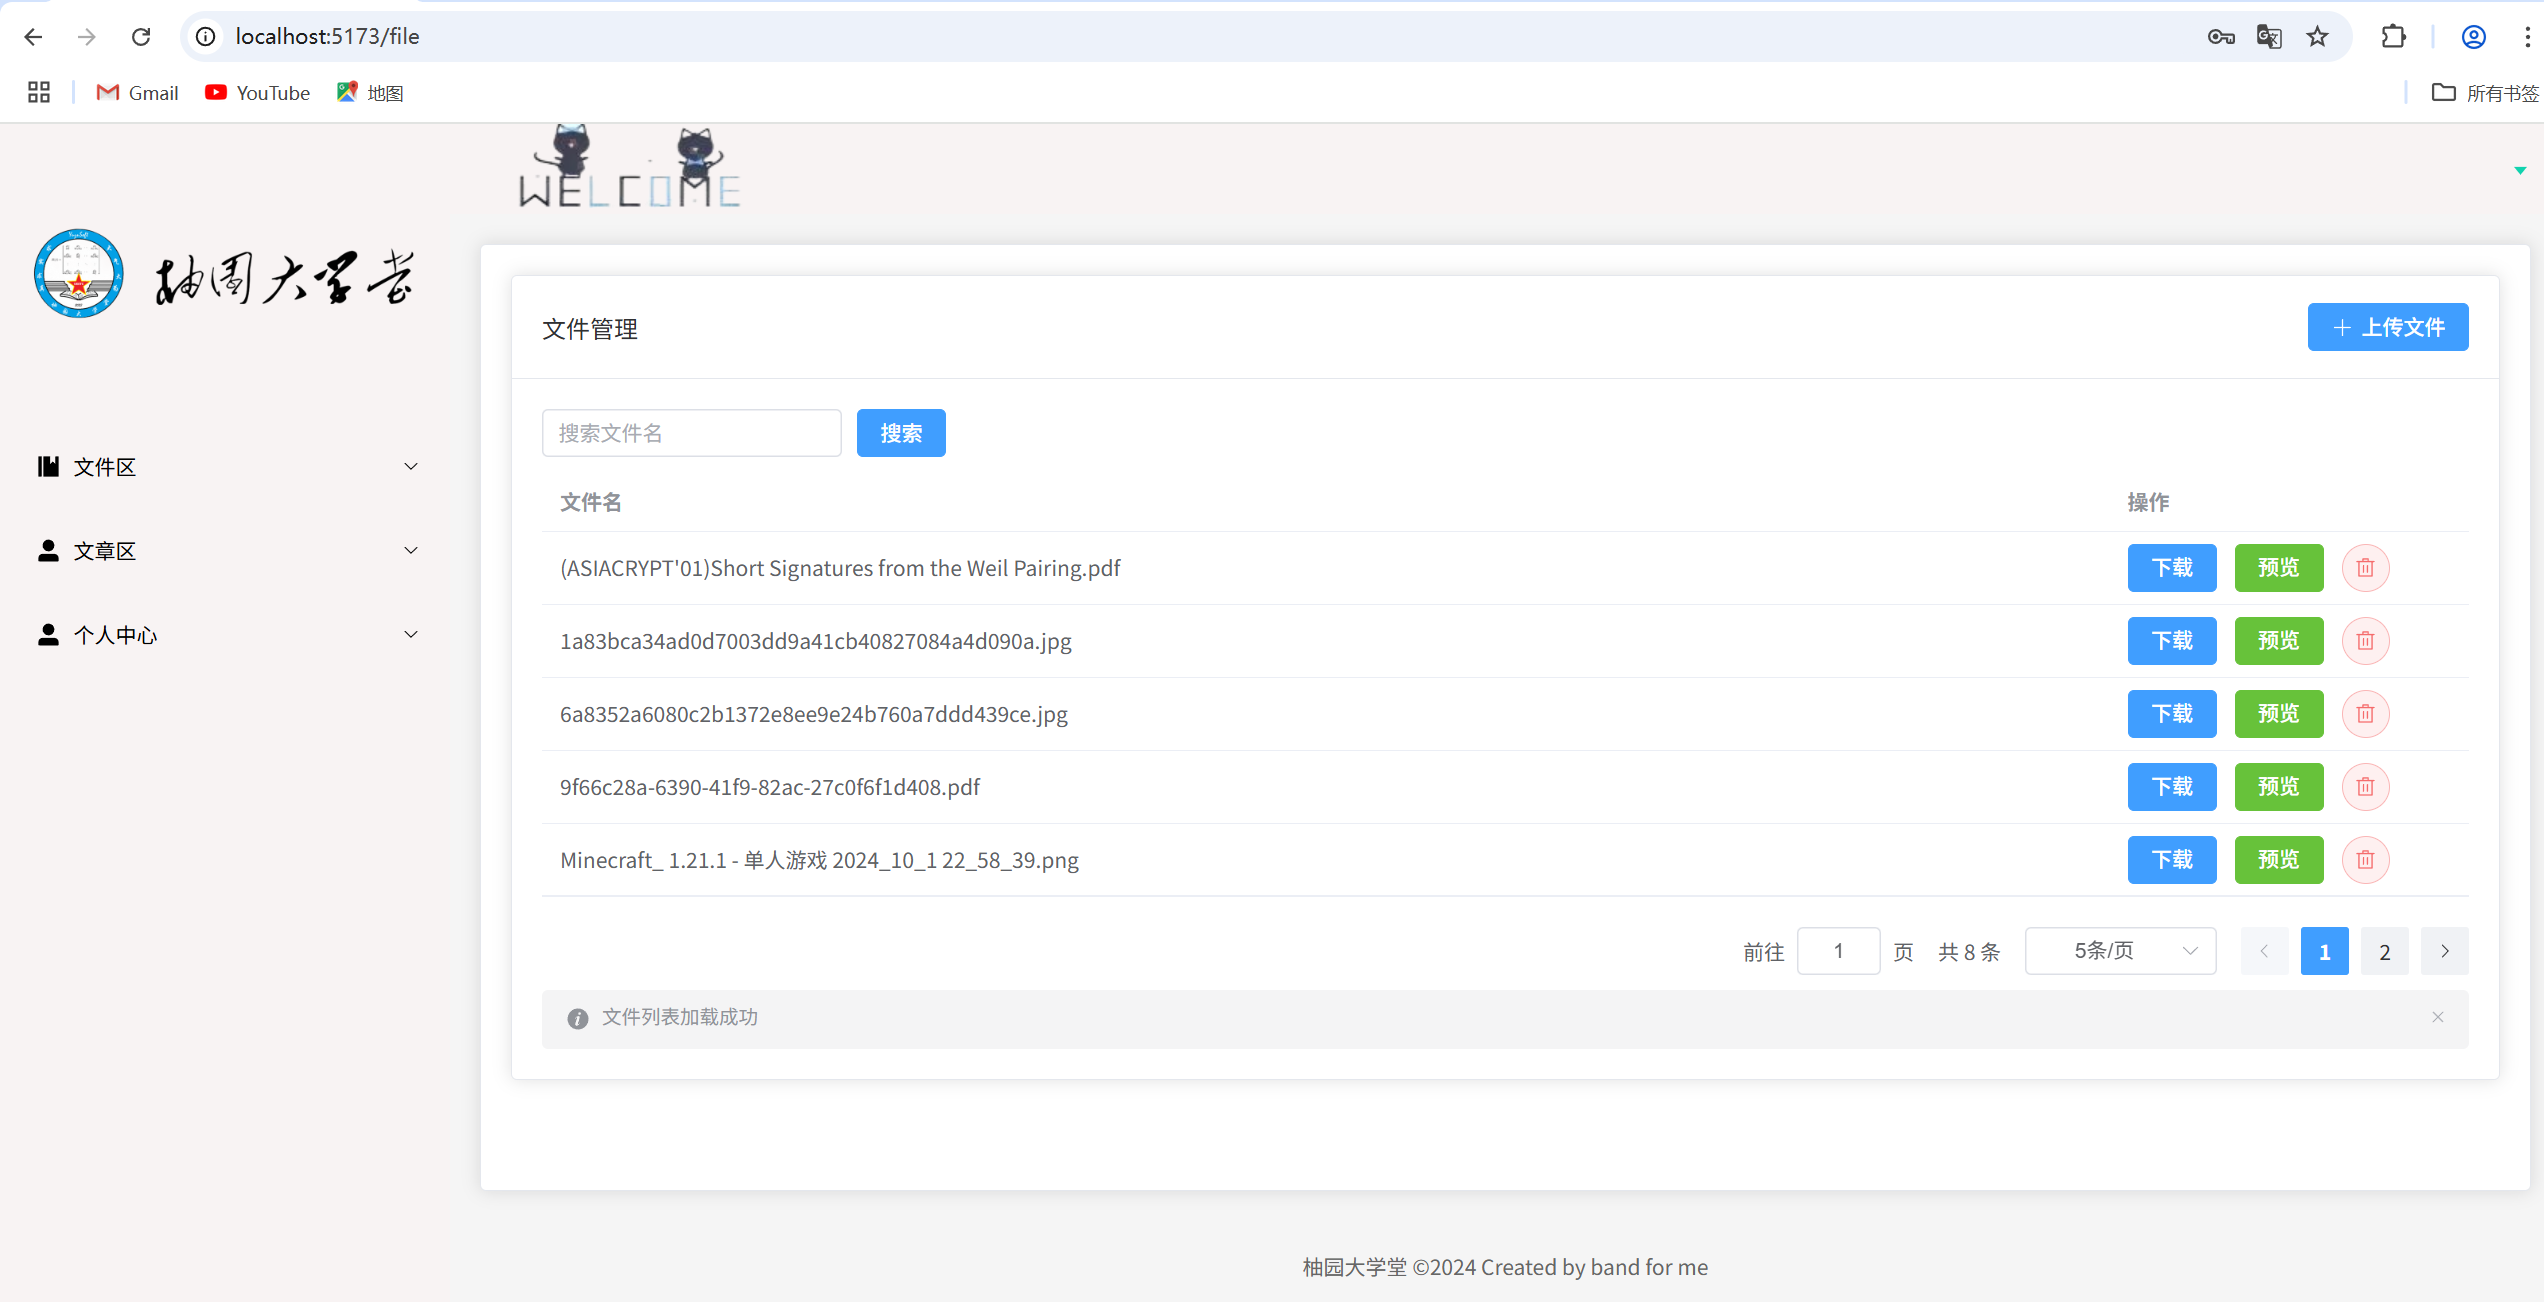
\includegraphics[width=0.5\textwidth]{主界面.png}
    \caption{主界面}
    \label{dc3}
\end{figure}

\subsection{用户信息更改}
用户信息更改,如图\ref{a1}所示。
\begin{figure}[htbp]
    \centering
    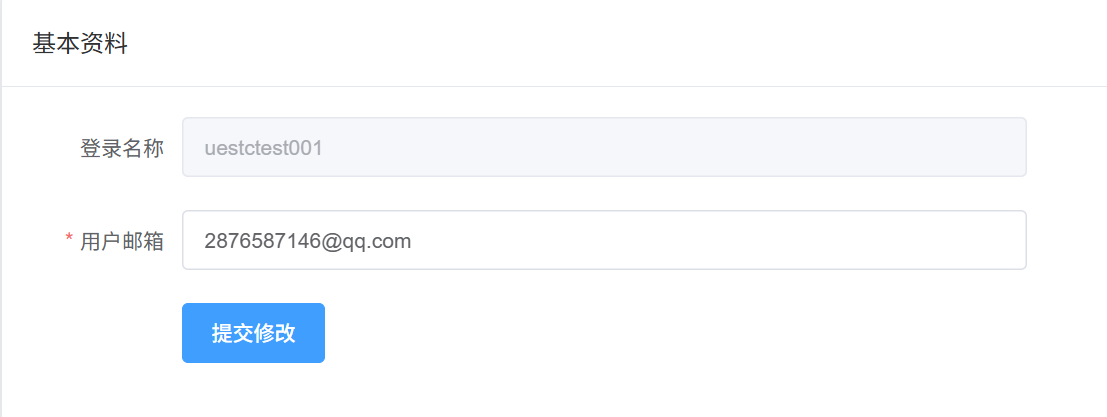
\includegraphics[width=0.5\textwidth]{用户信息.png}
    \caption{用户信息更改}
    \label{a1}
\end{figure}

用户信息更改前后对比,如图\ref{a1},\ref{a3}所示。
\begin{figure}[htbp]
    \centering
    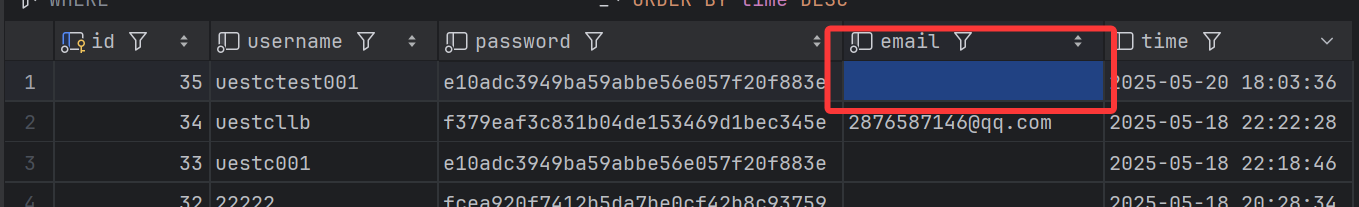
\includegraphics[width=0.5\textwidth]{用户信息更改前.png}
    \caption{修改前}
    \label{a2}
    
    \vspace{1em} % 两图之间留空,可调整
    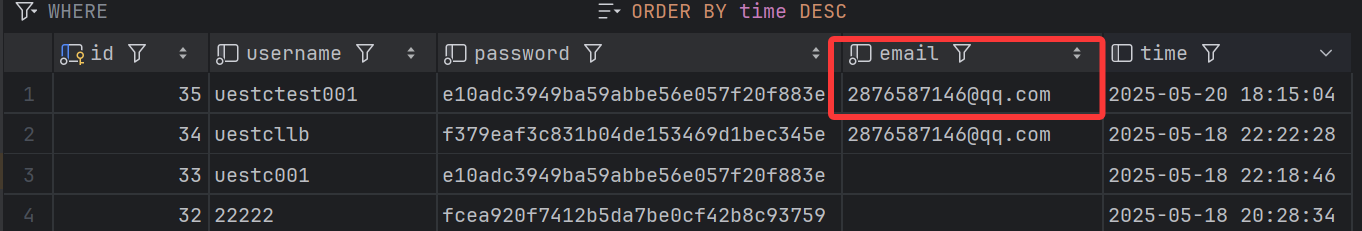
\includegraphics[width=0.5\textwidth]{用户信息更改后.png}
    \caption*{修改后} % 无编号标题,可改为caption{...}并加label
\end{figure}


\begin{figure}[htbp]
    \centering
    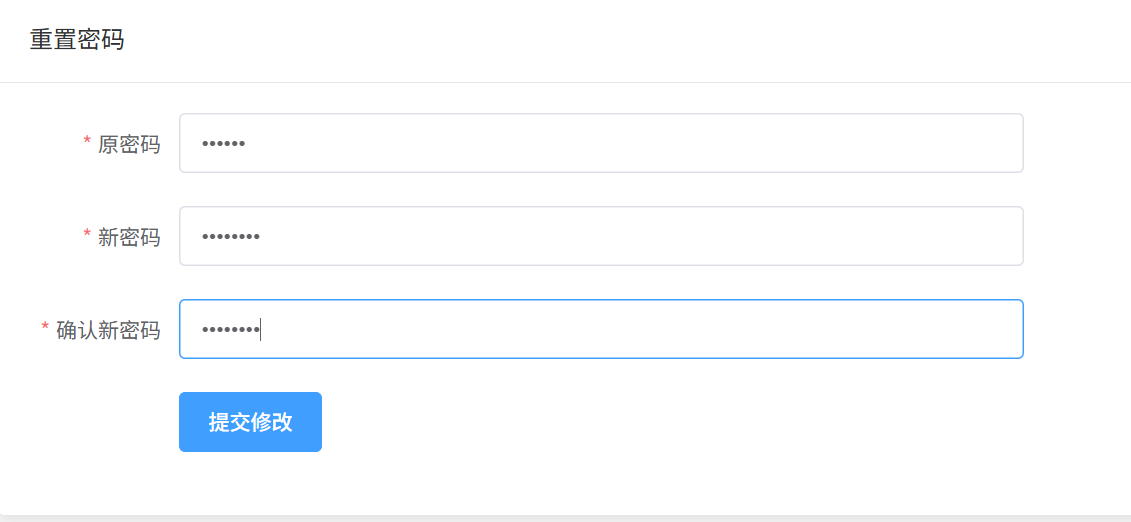
\includegraphics[width=0.5\textwidth]{密码1.png}
    \caption{更改密码界面}
    \label{a3}
\end{figure}
用户密码更改:
(原来为:123456,修改为:12345678)
可以看到密文已经发生了变化,说明密码已经被修改。如图\ref{a4}所示。
\begin{figure}[htbp]
    \centering
    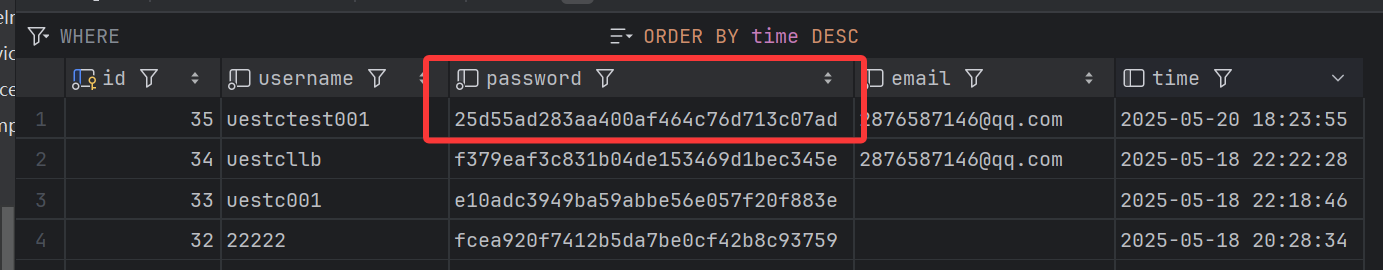
\includegraphics[width=0.5\textwidth]{密码2.png}
    \caption{数据库修改}
    \label{a4}
\end{figure}

\section{文章与文件区测试}
文章分类测试如图\ref{b1}所示。
文章上传测试如图\ref{b2}所示。
文章删除测试如图\ref{b3}所示。
文件上传测试如图\ref{c1}所示。
文件多种格式测试如图\ref{c2}所示。
文件下载测试如图\ref{c3}所示。
文件预览测试如图\ref{c4}所示。
文件删除测试如图\ref{c5}所示。

\begin{figure}[htbp]
    \centering
    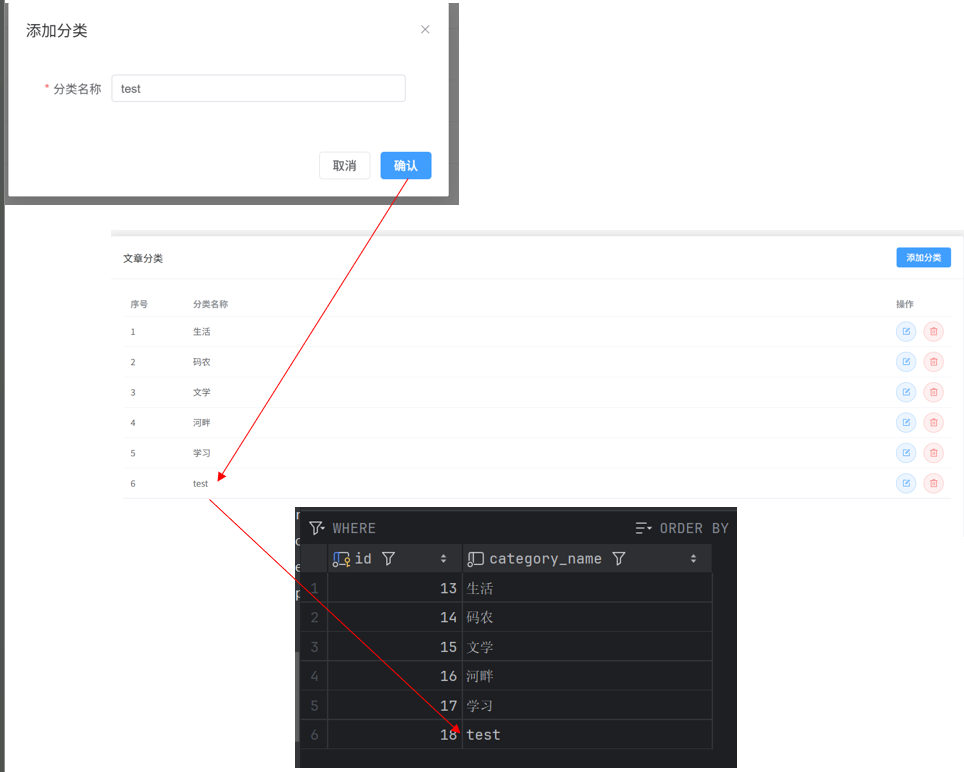
\includegraphics[width=0.7\textwidth]{分类.png}
    \caption{文章分类}
    \label{b1}
\end{figure}


\begin{figure}[htbp]
    \centering
    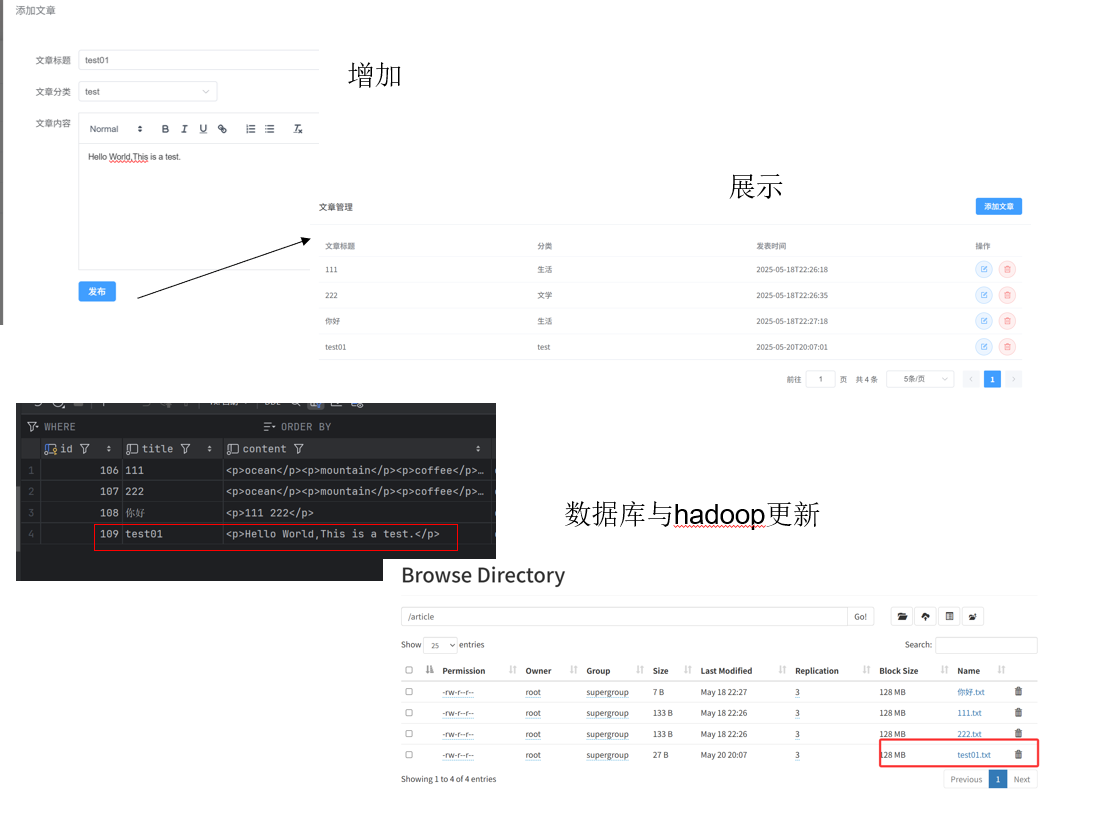
\includegraphics[width=0.7\textwidth]{文章上传.png}
    \caption{文章上传}
    \label{b2}
\end{figure}


\begin{figure}[htbp]
    \centering
    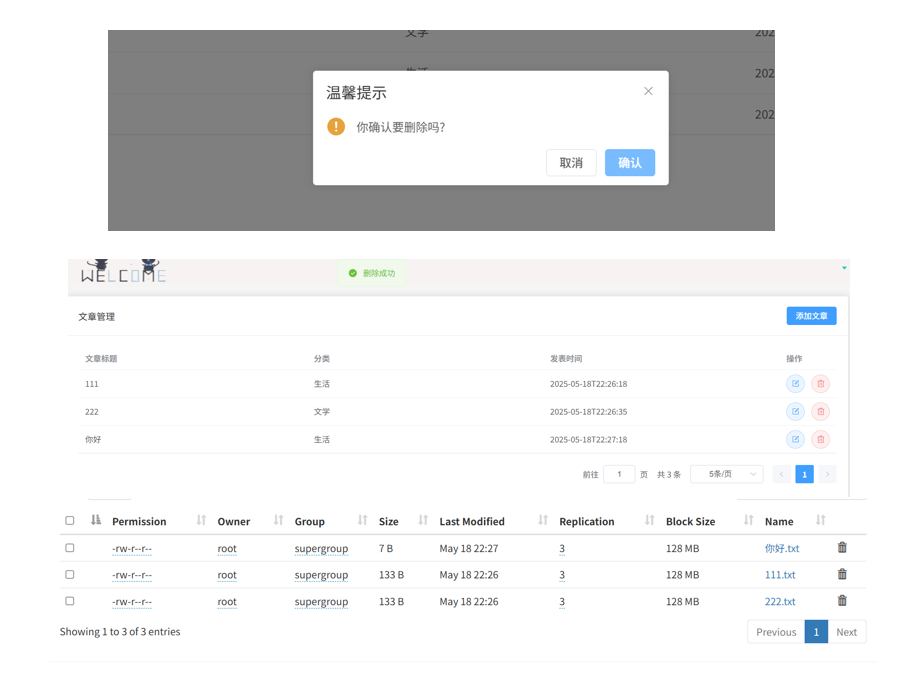
\includegraphics[width=0.7\textwidth]{文章删除.png}
    \caption{文章删除}
    \label{b3}
\end{figure}


\begin{figure}[htbp]
    \centering
    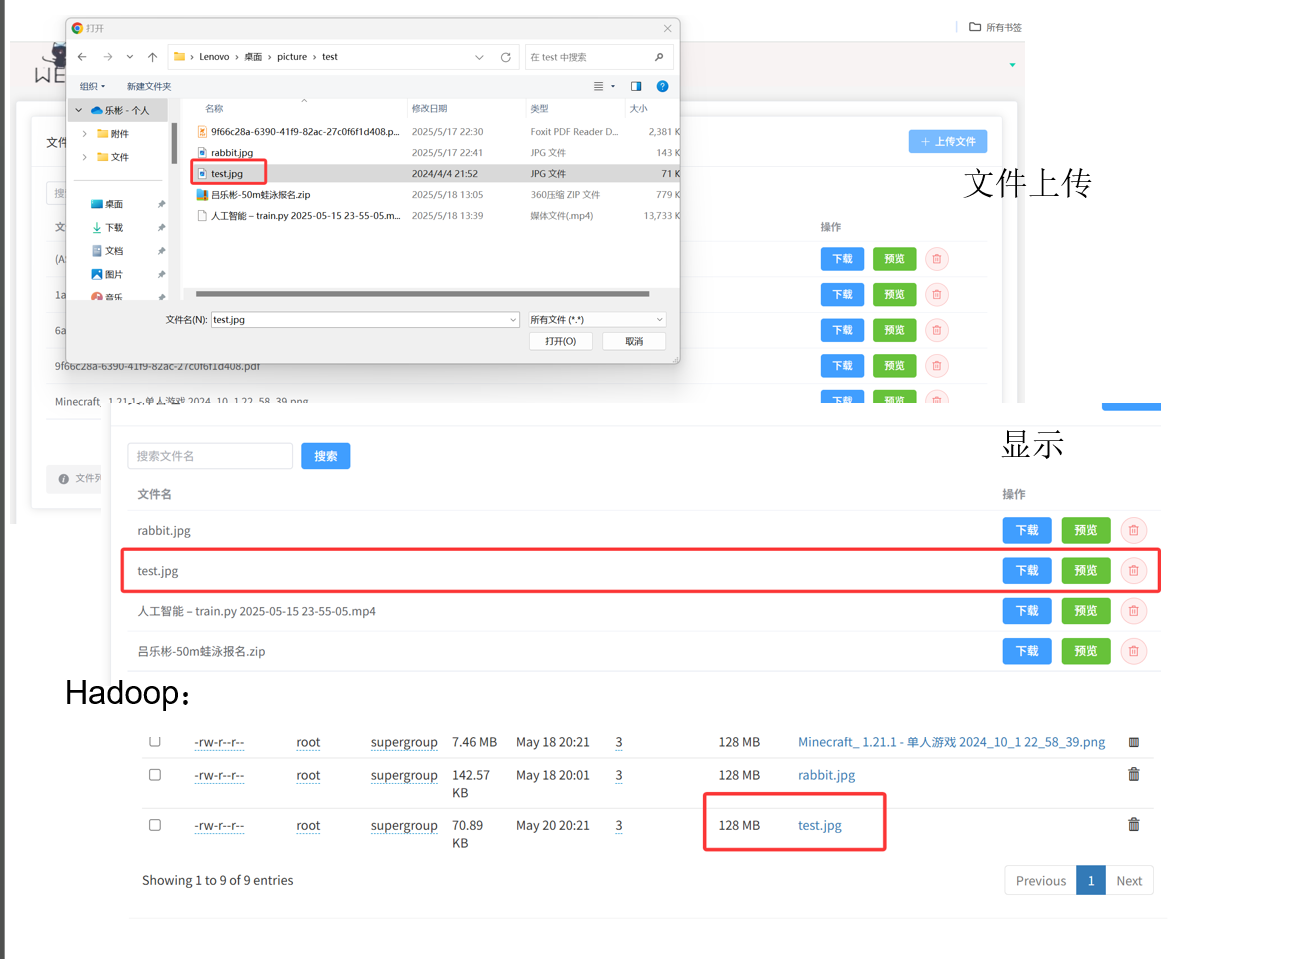
\includegraphics[width=0.7\textwidth]{文件上传.png}
    \caption{文件上传}
    \label{c1}
\end{figure}


\begin{figure}[htbp]
    \centering
    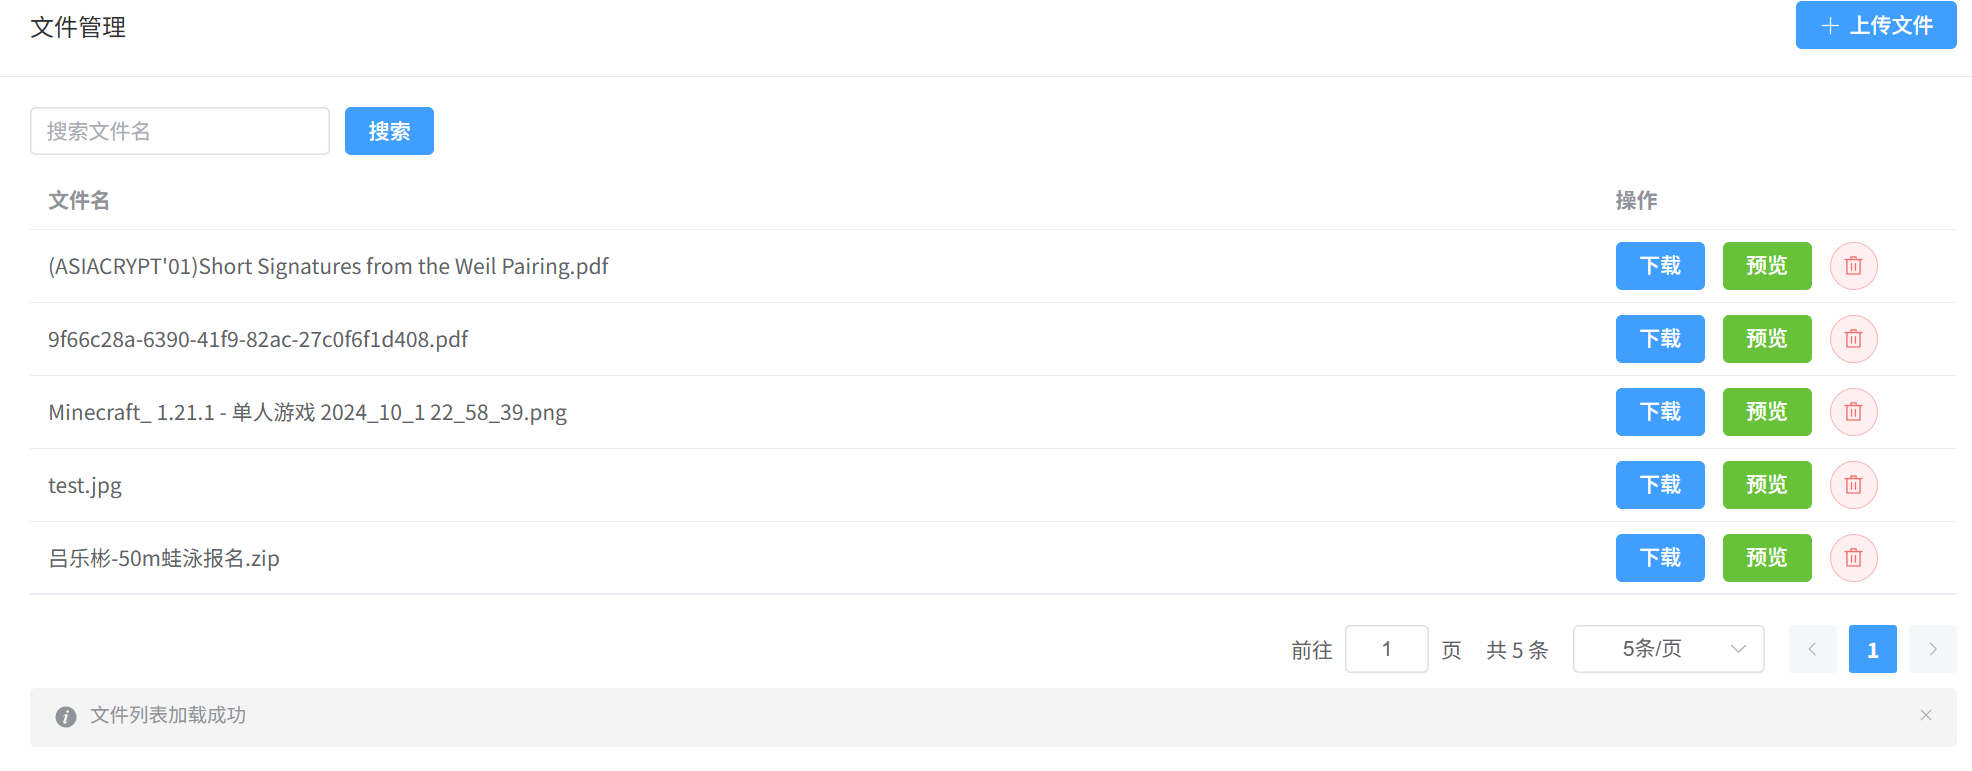
\includegraphics[width=0.7\textwidth]{文件格式.png}
    \caption{多种文件格式}
    \label{c2}
\end{figure}

\begin{figure}[htbp]
    \centering
    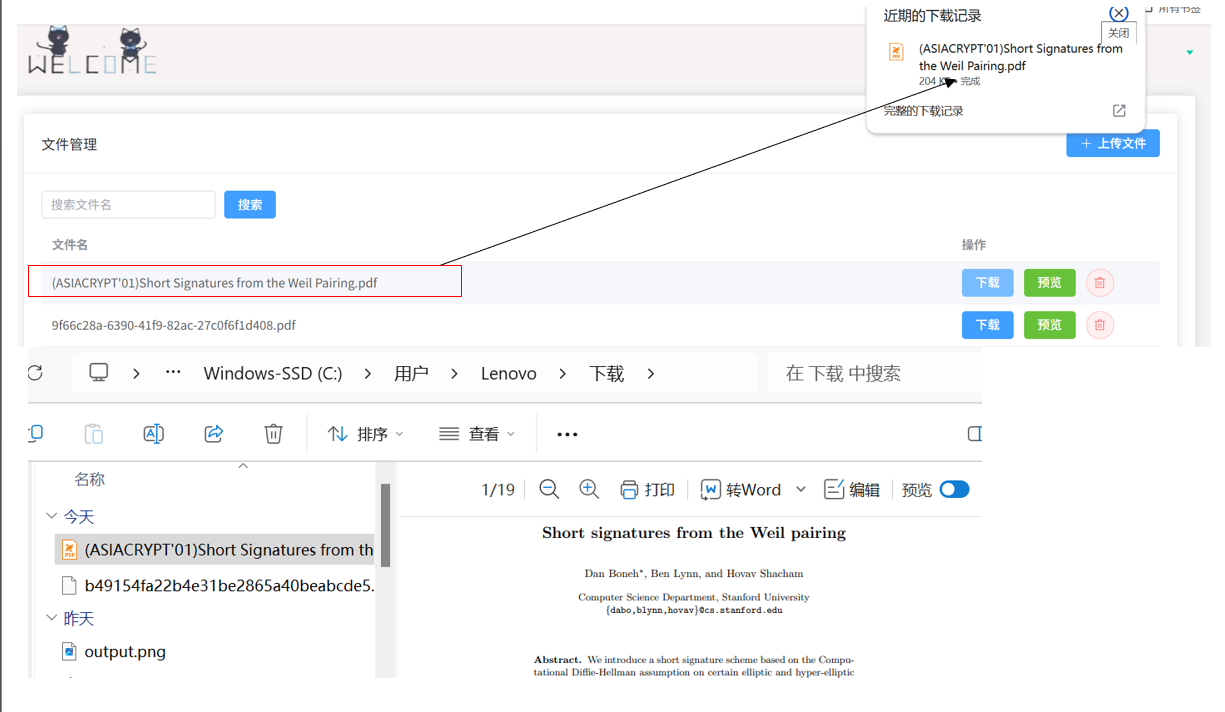
\includegraphics[width=0.7\textwidth]{文件下载.png}
    \caption{文件下载}
    \label{c3}
\end{figure}

\begin{figure}[htbp]
    \centering
    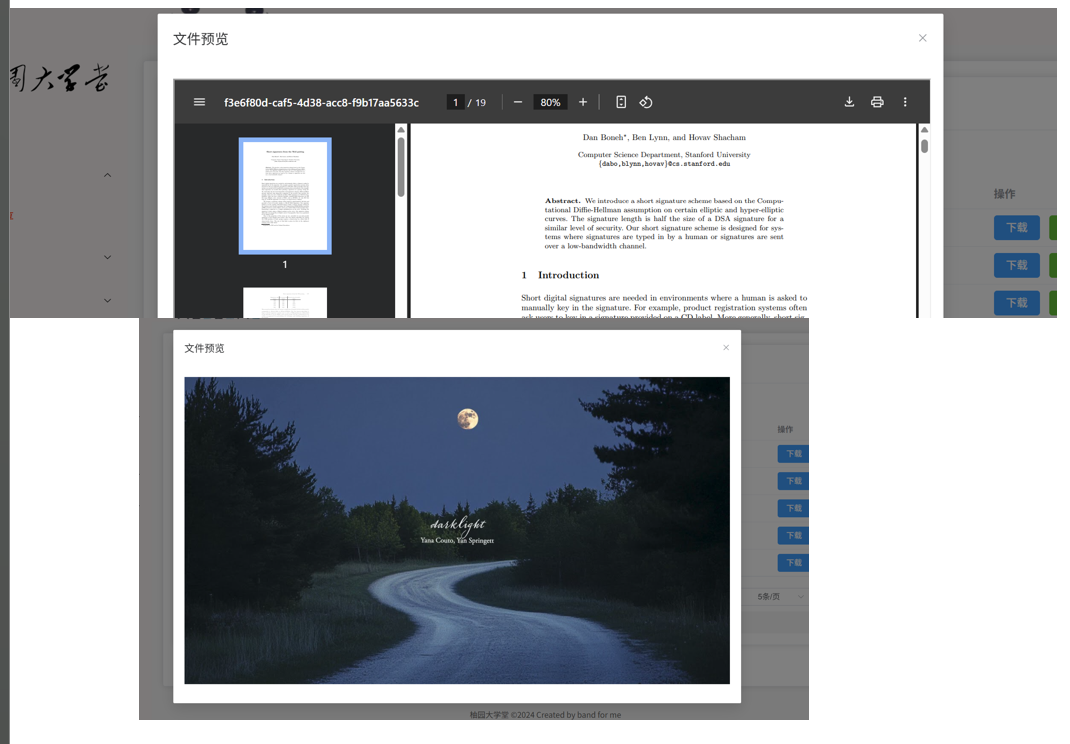
\includegraphics[width=0.7\textwidth]{文件预览.png}
    \caption{文件预览}
    \label{c4}
\end{figure}

\begin{figure}[htbp]
    \centering
    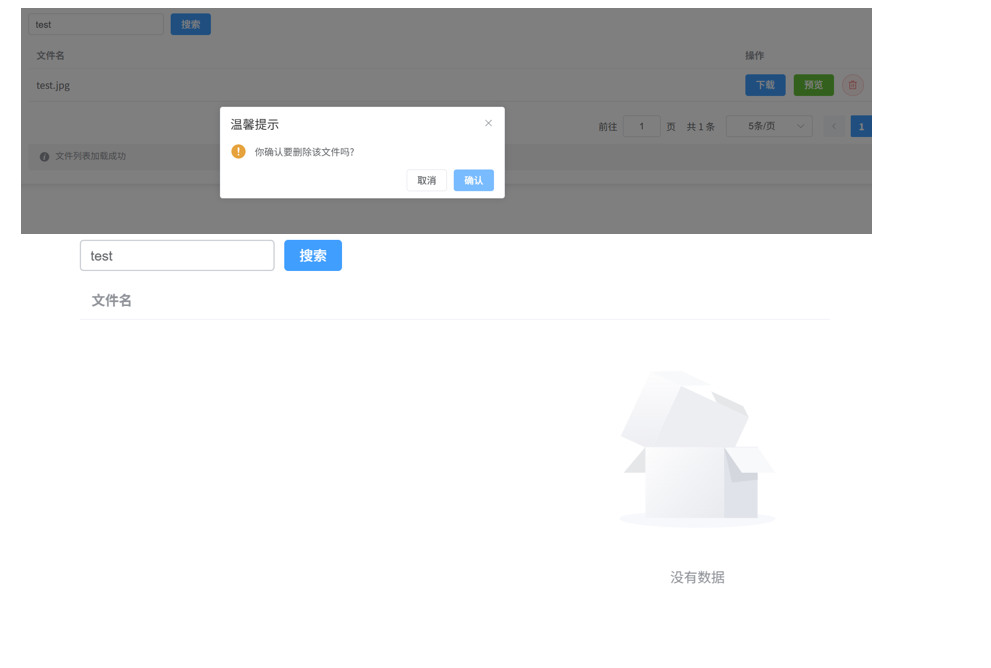
\includegraphics[width=0.7\textwidth]{文件删除.png}
    \caption{文件删除}
    \label{c5}
\end{figure}




\FloatBarrier % 添加命令
\section{小结}

本文围绕基于Hadoop HDFS的Web文件管理系统的设计
与实现进行了详细阐述。首先,介绍了系统的整体架构
和各模块的功能分工,包括Hadoop集群的搭建、
Spring Boot后端开发、Vue前端实现等关键环节。
随后,详细说明了系统的核心功能实现过程,
如文件与文章的增删改查、用户管理、权限控制
以及与Hadoop的集成方式。最后,通过功能测试
验证了系统的可用性和稳定性。

\bibliographystyle{unsrt}
\bibliography{reference}

\end{document}
